\chapter{Программный комплекс GADMA для вывода демографической истории популяций по генетическим данным и расширение библиотек \textit{stdpopsim} и \textit{demes}}
\label{ch:implementation}

В данной главе описаны программный комплекс GADMA, который реализует все разработанные модели и методы, а также расширение библиотек \textit{stdpopsim} и \textit{demes}, использованные для проведения экспериментальных исследований и представления результатов.

В разделе~\ref{sec:part5:gadma} приведено описание программного комплекса GADMA (Global search Algorithm for Demographic Model Analysis).
Все экспериментальные исследования методов в данной работе были проведены с использованием этого программного комплекса.
Приведена структура комплекса и ее основные компоненты, часть которых была описана ранее.

Раздел~\ref{sec:part5:gadma} включает описание существующих библиотек \textit{stdpopsim} и \textit{demes}, которые были расширены для использования в данной работе.
Библиотека \textit{stdpopsim} позволяет проводить симуляции генетических данных с использованием каталога видов и их демографических историй.
Основное назначение библиотеки \textit{demes} в текстовом и визуальном представлении демографических историй.
Все изображения историй в данной работе были получены с использованием \textit{demes}.

\section{Программный комплекс GADMA для вывода демографической истории популяций по генетическим данным}
\label{sec:part5:gadma}

Все разработанные модели и методы были реализованы в программном комплексе GADMA.
Основным назначением GADMA является повышение эффективности, а также снижение уровня сложности процесса вывода демографической истории популяций по генетическим данным.
Программный комплекс GADMA с открытым исходным кодом доступен в репозитории~\url{https://github.com/ctlab/GADMA}.
Его документация доступна \url{https://gadma.readthedocs.io}.

Программный комплекс включает в себя набор методов настройки параметров моделей и «движков» --- методов вычисления правдоподобия.
Всего реализованы четыре «движка», которые соответствуют существующим методам: \dadi, \moments, \momi, \momentsLD.
Программный комплекс имеет два режима:
\begin{enumerate}
    \item Режим заданной модели. В этом режиме пользователь самостоятельно задает интересующую его модель демографической истории популяций. Комплекс GADMA настраивает параметры заданной модели.
    \item Режим автоматического перебора моделей. Пользователь задает минимальные и максимальные ограничения на модели, а GADMA производит автоматический перебор моделей в пределах заданных ограничений, настраивает их параметры и выбирает наилучшую модель. 
\end{enumerate}

Для запуска GADMA пользователю достаточно выбрать режим, движок и метод настройки параметров моделей.

\subsection{Структура программного комплекса GADMA}

\begin{figure}[ht]
    \centering
    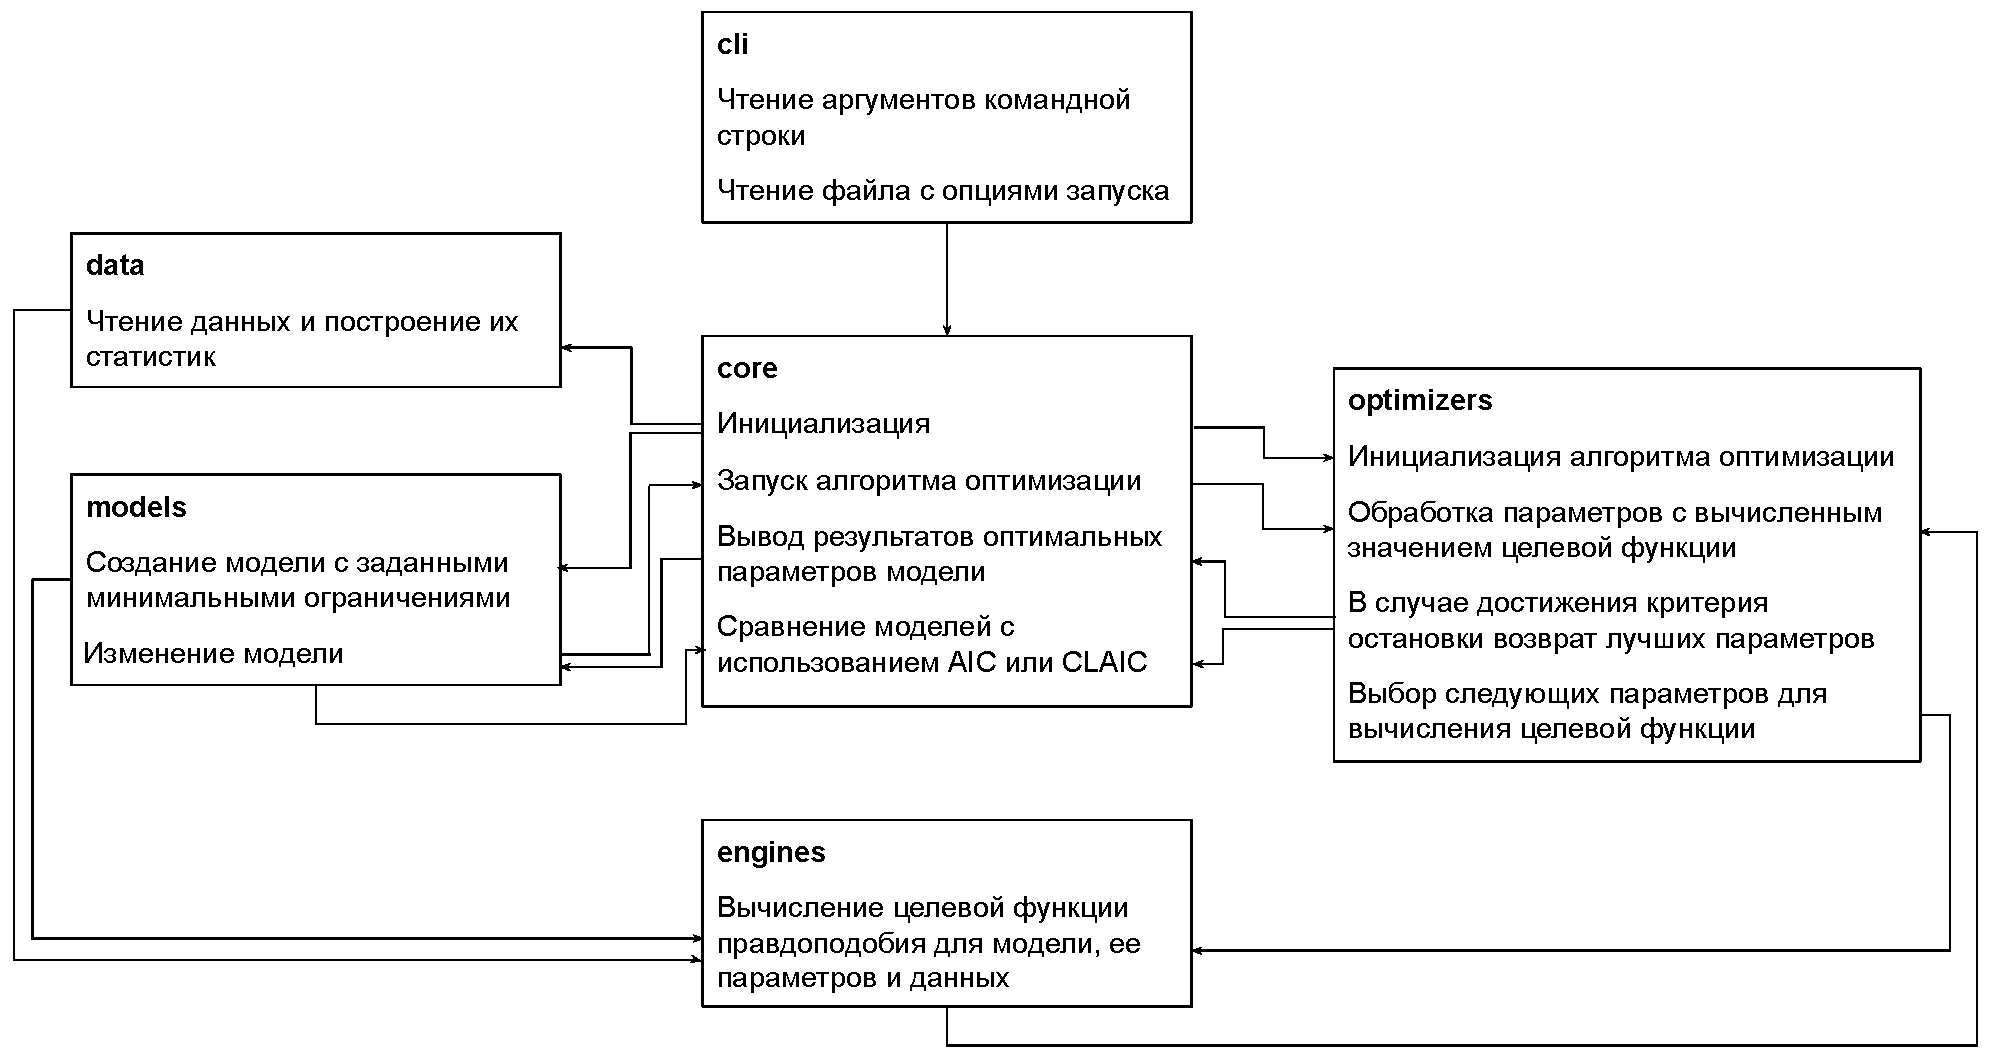
\includegraphics[width=\linewidth]{images/part5/gadma_modules.pdf}
    \caption{Структура программного комплекса GADMA}
    \label{fig:part5:gadma_modules}
\end{figure}

На рисунке~\ref{fig:part5:gadma_modules} приведена общая структура программного комплекса.
Она включает в себя шесть основных модулей: \texttt{core}, \texttt{cli}, \texttt{data}, \texttt{models}, \texttt{engines} и \texttt{optimizers}.

\textbf{Модуль \texttt{core} }является входной точкой программного комплекса и управляет остальными модулями.
Основными входными данными является аргументы командной строки и файл с опциями для запуска.
Чтение входных данных происходит в \textbf{модуле \texttt{cli}} и возвращается в корневой модуль.
Затем происходит инициализация согласно полученным опциям.
Происходит чтение генетических данных с помощью модуля \texttt{data} и создание модели демографической истории согласно опциям, выбранным пользователем.
Если выбран режим заданной модели, то именно она и анализируется.
В противном случае при выборе режима автоматического перебора создается модель, соответствующая минимальным ограничениям, которая в дальнейшем будет изменяться.
Затем происходит запуск метода оптимизации из модуля \texttt{optimizers}, который возвращает настроенные параметры модели.
Модуль выводит найденные параметры.
Если был выбран режим автоматического перебора, то следует обращение к модулю \texttt{models} для изменения модели и затем снова происходит запуск метода оптимизации.
Так повторяется до тех пор, пока не будет достигнуты максимальные ограничения на модели.
В конце работы в режиме автоматического перебора модуль \texttt{core} сравнивает все полученные модели с использованием метрик AIC или CLAIC.
Выбор метрики зависит от наличия зависимостей в данных --- информация, которая указывается пользователем.

%\subsection{Модуль \texttt{data}}

\textbf{Модуль \texttt{data}} содержит инструменты для работы и хранения генетических данных.
Он позволяет прочитать генетические данные, которые могут быть представлены в разных форматах, и строит по ним статистики для дальнейшего использования такие, как аллель-частотный спектр или статистики неравновесного сцепления генов.
Подробное описание этих статистик представлено в разделе~\ref{sec:part1:dem_inf:data_stats}.
Рисунок~\ref{fig:part5:data_classes} показывает структуру классов модуля.
Абстрактный класс \texttt{DataHolder} хранит указатель на генетические данные.
Класс \texttt{VCFDataHolder} хранит генетические данные в формате VCF~\cite{danecek2011variant}.
Класс \texttt{SFSDataHolder} позволяет хранить указатель на файл с аллель-частотным спектром, который может быть в нескольких форматах~\cite{gutenkunst2009inferring,kamm2020efficiently,excoffier2013robust}.

\begin{figure}[ht]
    \centering
    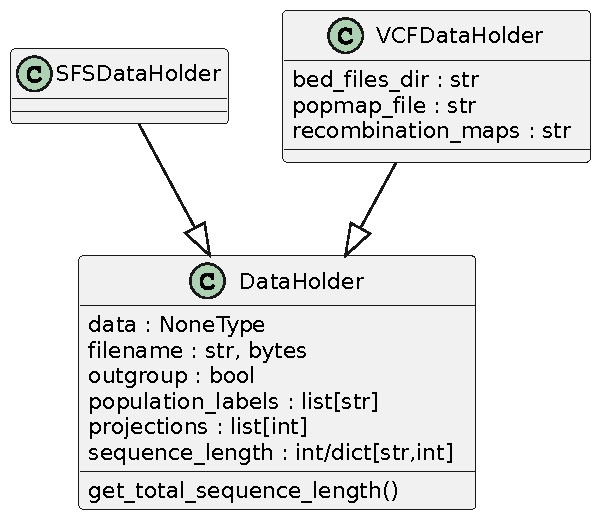
\includegraphics[width=0.3\linewidth]{images/part5/data_classes.pdf}
    \caption{Структура классов модуля \texttt{data} программного комплекса GADMA}
    \label{fig:part5:data_classes}
\end{figure}

%\subsection{Модуль \texttt{models}}
\textbf{Модуль \texttt{models}} предназначен для создания и хранения моделей.
Он уже был описан ранее в разделах~\ref{sec:part2:new_models}~и~\ref{sec:part4:implementation}.
Структура классов была представлена на рисунках~\ref{fig:part2:model_classes}~и~\ref{fig:part4:auto_method_impl}.
%На рисунке~\ref{fig:part5:model_classes} приведена полная структура классов модуля \texttt{models}.


% \begin{figure}[ht]
%     \centering
%     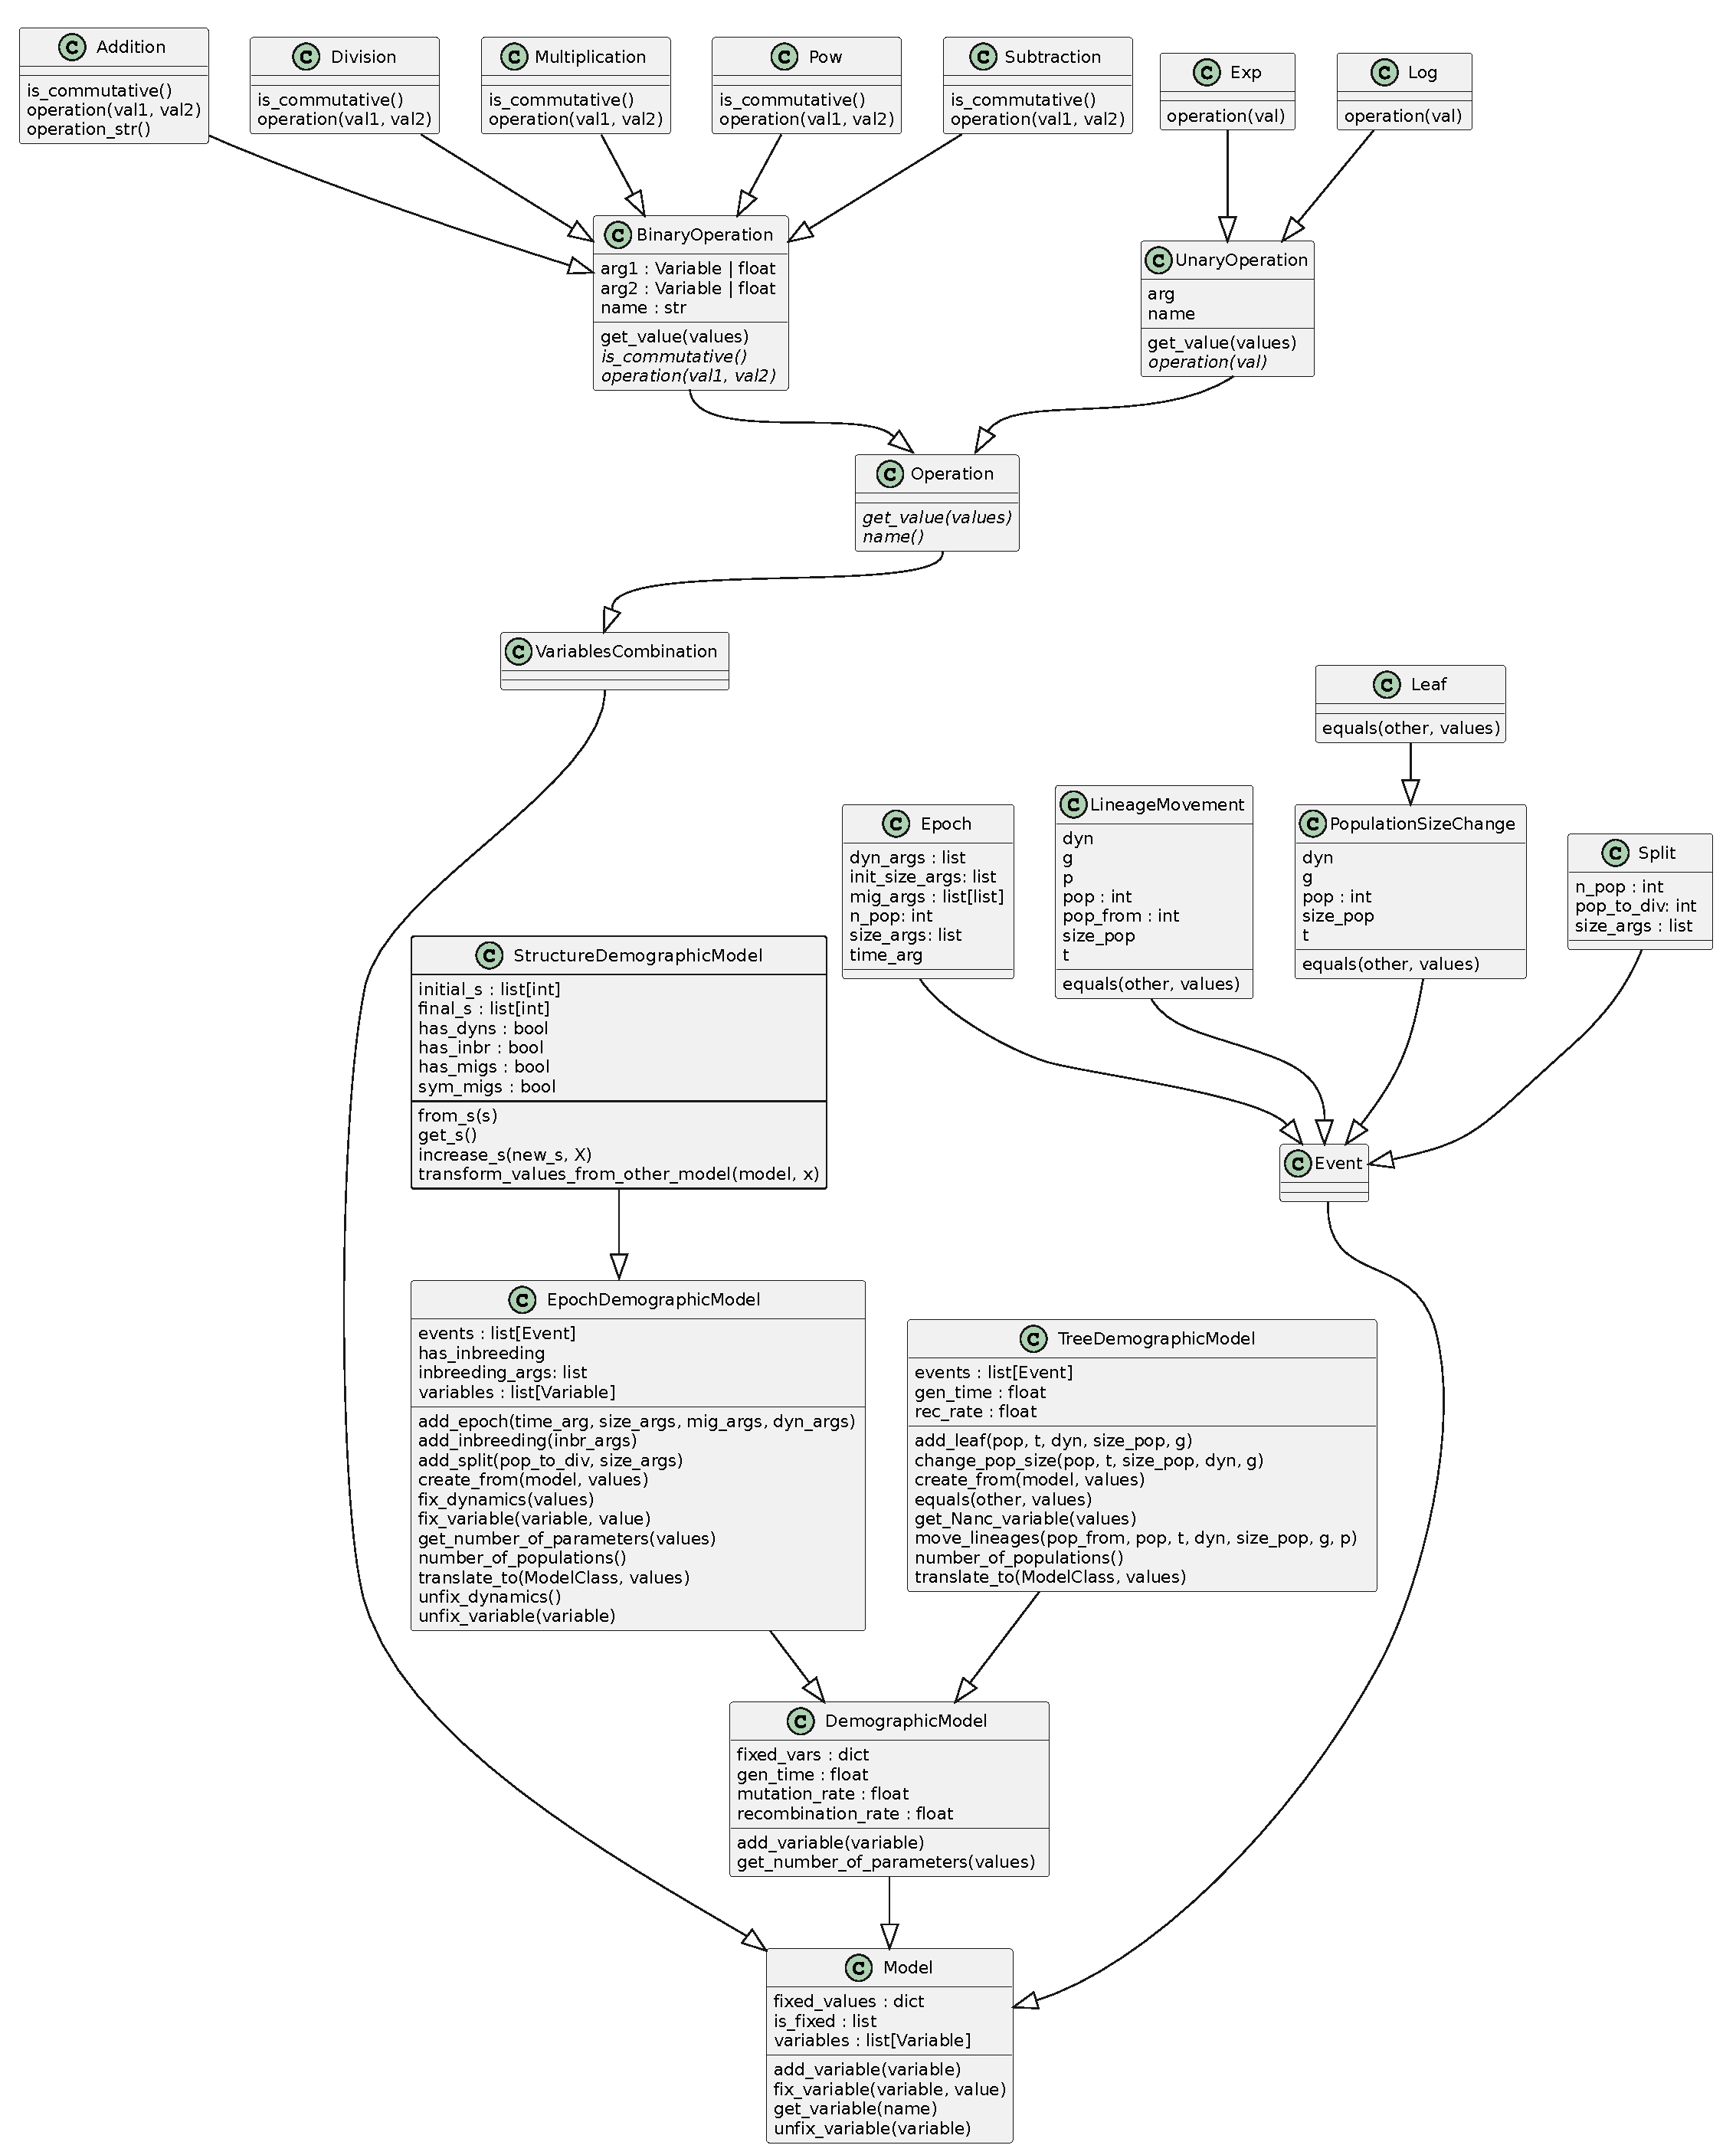
\includegraphics[width=\linewidth]{images/part5/models_full_classes.pdf}
%     \caption{Структура классов модуля \texttt{models} программного комплекса GADMA}
%     \label{fig:part5:model_classes}
% \end{figure}

%\subsection{Модуль \texttt{optimizers}}

\textbf{Модуль \texttt{optimizers}} содержит методы настройки параметров моделей по генетическим данным.
На рисунке~\ref{fig:part2:bayesian_optimization:implementation:bo} ранее была представлена структура классов этого модуля.
Модуль реализует метод на основе комбинации методов глобальной и локальной оптимизации.
На выбор пользователя представлены следующие методы глобальной оптимизации:
\begin{itemize}
    \item генетический алгоритм, описанный в разделе~\ref{sec:part2:genenic_algorithm} и реализованный классом \texttt{GeneticAlgorithm};
    \item байесовская оптимизация, описанная в разделе~\ref{sec:part2:bayesian_optimization} и реализованная классами \texttt{SMACBayesianOptimizer} и \texttt{SMACBOEnsemble}.
\end{itemize}
GADMA предоставляет выбор из следующих методов локальной оптимизации:
\begin{itemize}
    \item метод BFGS;
    \item метод L-BFGS-B;
    \item метод Пауэлла;
    \item метод Нелдера-Мида.
\end{itemize}


% \begin{figure}[ht]
%     \centering
%     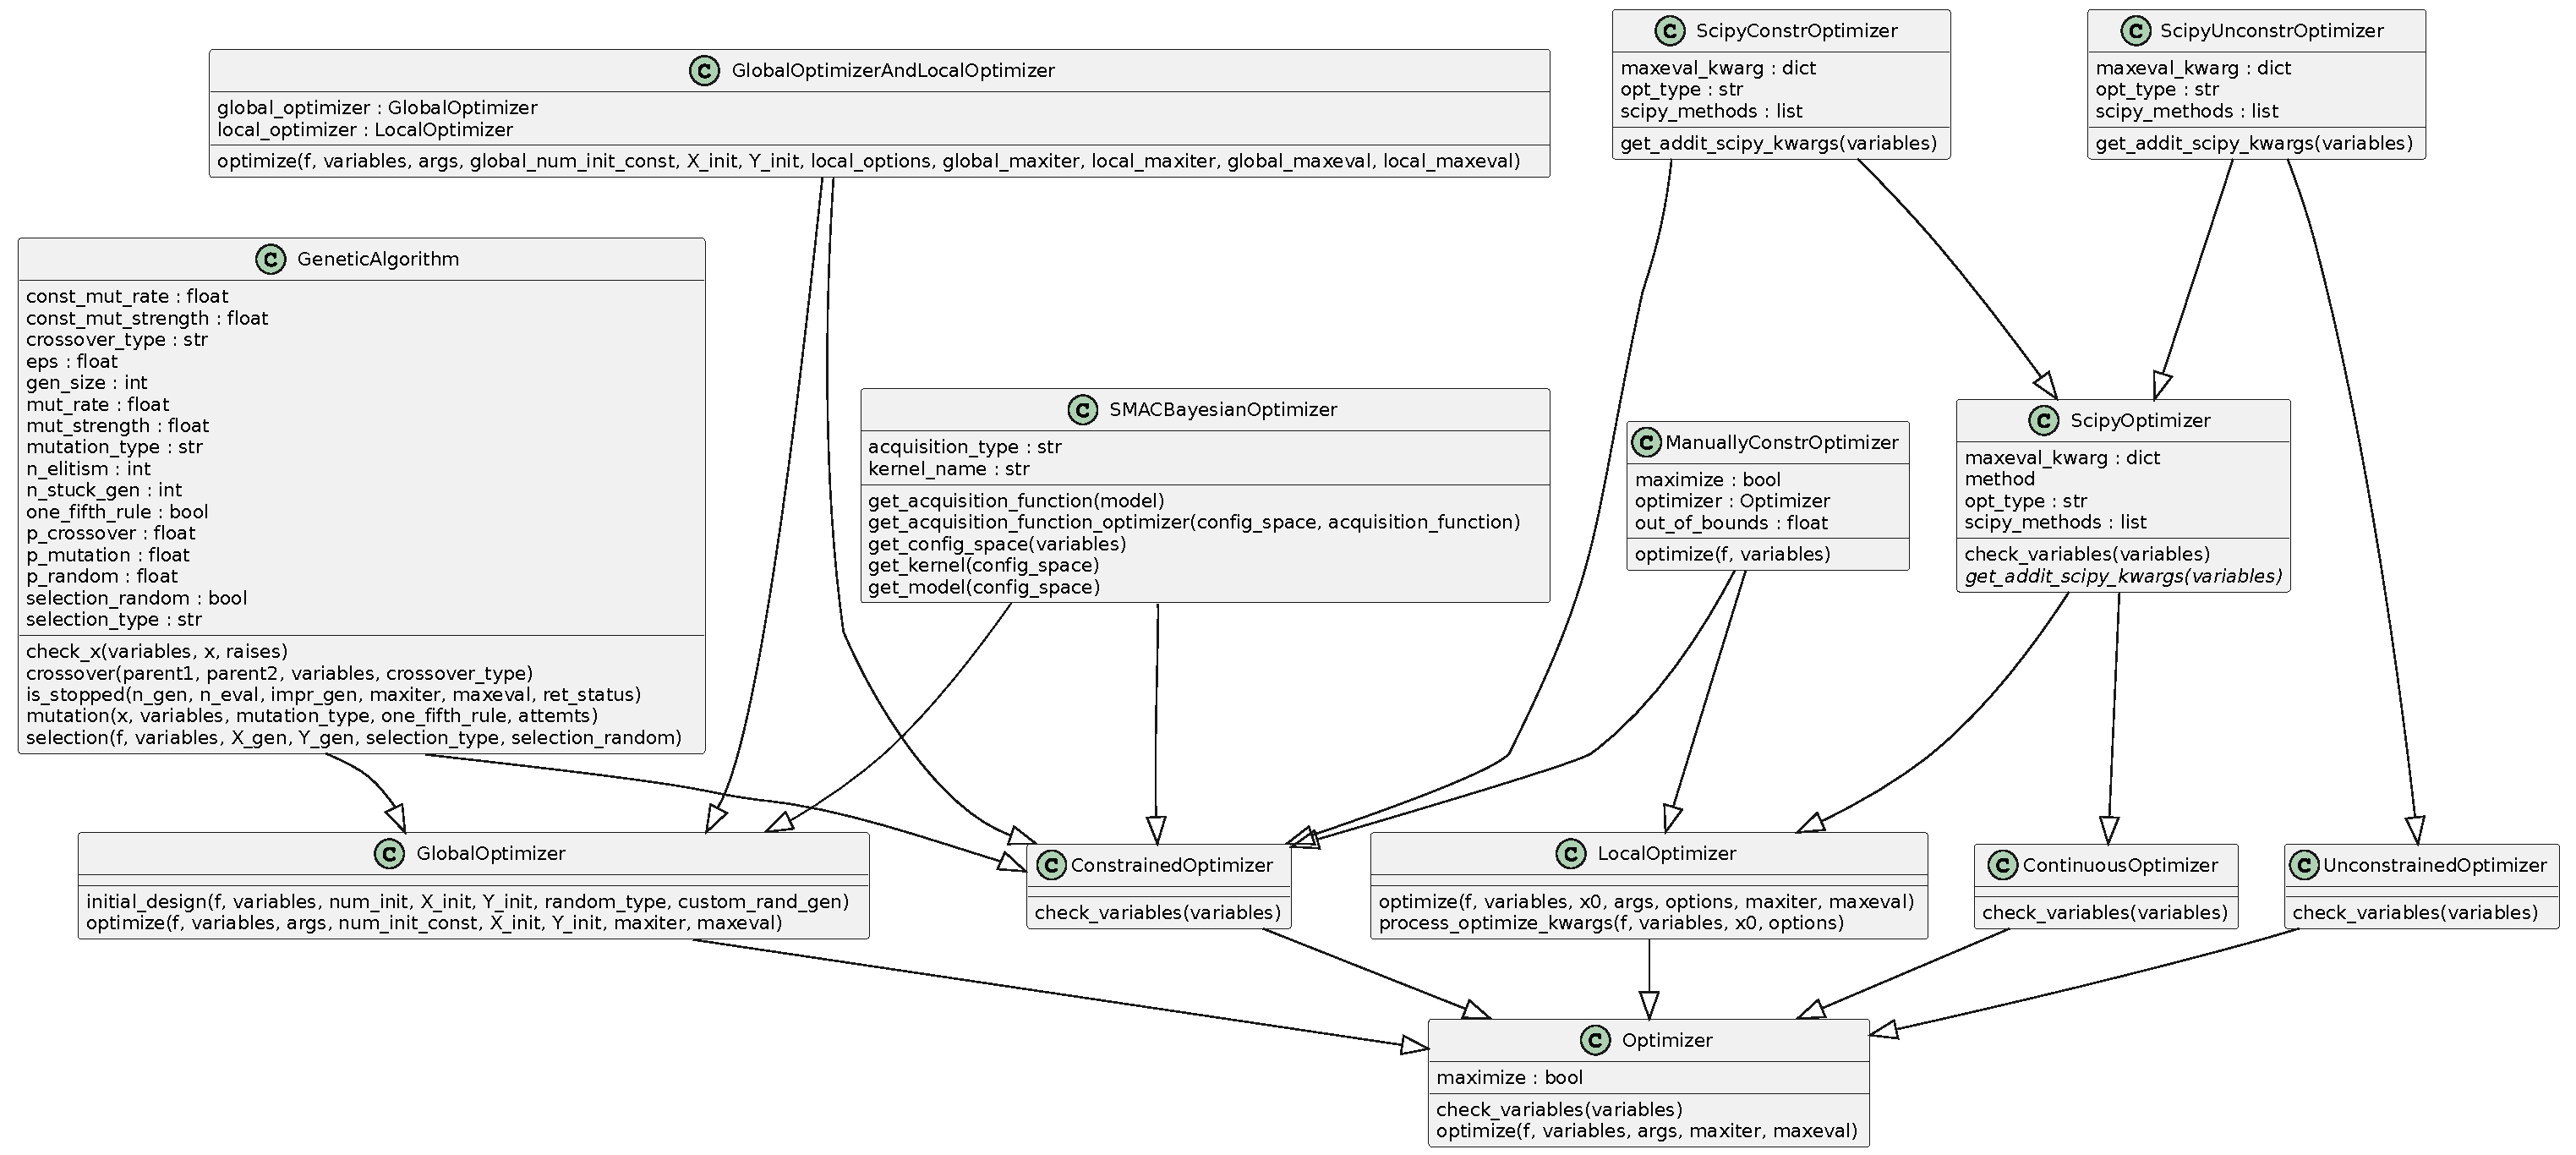
\includegraphics[width=\linewidth]{images/part5/optimizer_classes.pdf}
%     \caption{Структура классов модуля \texttt{optimizer} программного комплекса GADMA}
%     \label{fig:part5:optimizer_classes}
% \end{figure}

%\subsection{Модуль \texttt{engines}}

\textbf{Модуль \texttt{engines}} включает реализацию движков GADMA --- методов вычисления правдоподобия, которые используются методами оптимизации для настройки параметров моделей по генетическим данным.
Структура классов представлена на рисунке~\ref{fig:part5:engines_classes}.

\begin{figure}[ht]
    \centering
    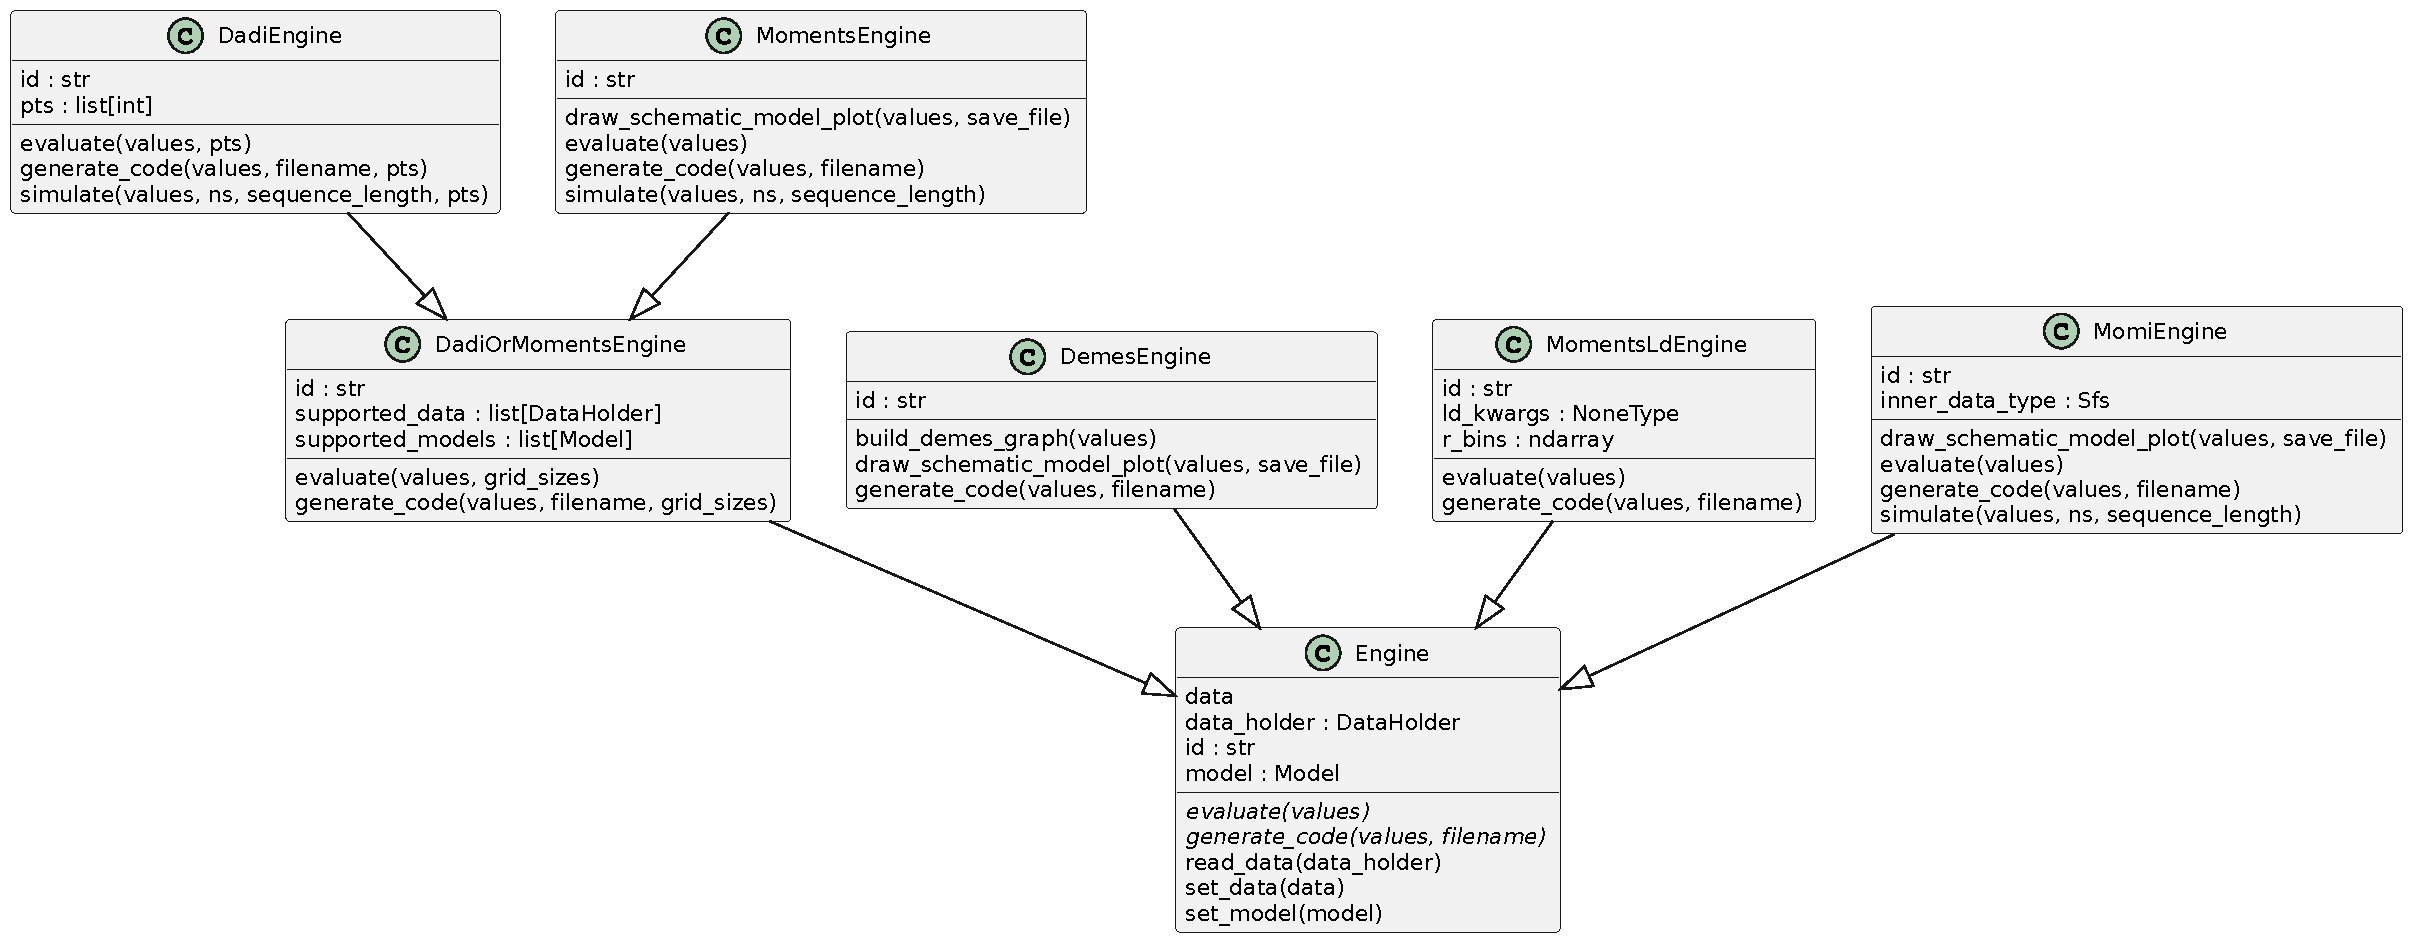
\includegraphics[width=\linewidth]{images/part5/engine_classes.pdf}
    \caption{Структура классов модуля \texttt{engines} программного комплекса GADMA}
    \label{fig:part5:engines_classes}
\end{figure}

Модуль включает абстрактный класс \texttt{Engine}, от которого наследуются все движки.
Объекты этого класса имеют атрибут \texttt{id} для идентификации движка, генетические данные \texttt{data\_holder}, представленные объектом класса \texttt{DataHolder} и атрибут \texttt{model} заданной модели демографической истории популяций, являющейся объектом класса \texttt{Model}.
Основной процедурой класса \texttt{Engine} является абстрактная процедура \texttt{evaluate}, которая вычисляет значение правдоподобия генетических данных при условии модели с заданными параметрами \texttt{values}.
Процедура \texttt{generate\_code} генерирует спецификацию модели с заданными параметрами с использованием интерфейса движка.
Например, для движка \texttt{dadi} --- это будет процедура для языка программирования Python, пример которой показан на рисунке~\ref{fig:dadi:model_spec}.

Программный комплекс GADMA реализует четыре движка для вычисления правдоподобия:
\begin{itemize}
    \item движок \texttt{dadi}, реализующий метод аппроксимации диффузией библиотеки \dadi~--- класс \texttt{DadiEngine};
    \item движок \texttt{moments}, реализующий метод моментов для аллель-частотного спектра библиотеки \moments~--- класс \texttt{momentsEngine};
    \item движок \texttt{momi2}, реализующий метод непрерывной модели Морана библиотеки \momi~--- класс \texttt{MomiEngine};
    \item движок \texttt{momentsLD}, реализующий метод моментов для статистик неравновесного сцепления генов библиотеки \momentsLD~--- класс \texttt{MomentsLdEngine}.
\end{itemize}

Один дополнительный движок \texttt{demes}, реализованный классом \texttt{DemesEngine}, включен в GADMA для визуального представления демографических историй.
Он использует библиотеку \demes, которая будет описана далее.
Для рисования демографических историй используется процедура \texttt{draw\_schematic\_model\_plot}.
GADMA предоставляет выбор из трех движков для визуального представления демографических историй:
\begin{itemize}
    \item движок \texttt{moments};
    \item движок \texttt{momi2};
    \item движок \texttt{demes}.
\end{itemize}

\subsection{Входные данные и интерфейс запуска}

На вход программный комплекс GADMA принимает файл с опциями запуска, список которых с описанием приведен в таблице~\ref{tab:part5:input}.
Запуск GADMA для заданного файла \texttt{params\_file} с опциями выполняется из командной строки следующим образом:

\texttt{\$ gadma -p params\_file}\\

Пример входного файла с опциями изображен на рисунке~\ref{fig:part5:input_example}.

\begin{table}[!htbp]
    \centering
    \resizebox{\linewidth}{!}{%
    \begin{tabular}{|p{4.3cm}|p{8cm}|}
        \hline
        \texttt{Output directory} & Директория для записи результатов\\
        \hline
        \multicolumn{2}{|c|}{\textbf{Информация о генетических данных}} \\
        \hline
        \texttt{Input data} & Путь к файлу с генетическими данными\\
        \hline
        \texttt{Population labels} & Названия рассматриваемых популяций\\
        \hline
        \texttt{Projections} & Число образцов для каждой популяции\\
        \hline
        \texttt{Sequence length} & Длина представленной последовательности\\
        \hline
        \texttt{Linked SNP's} & Информация о наличии или отсутствии зависимостей в генетических данных, которая используется для выбора AIC или CLAIC \\
        \hline
        \texttt{Directory with bootstrap} & Директория с множеством сгенерированных данных для вычисления CLAIC \\
        \hline
        \multicolumn{2}{|c|}{\textbf{Информация о популяциях}} \\
        \hline
        \texttt{Mutation rate} & Скорость мутации одной позиции генома на одно поколение\\
        \hline
        \texttt{Recombination rate} & Вероятность рекомбинации между позициями генома, расположенными на расстоянии миллиона пар оснований\\
        \hline
        \texttt{Time for generation} & Среднее время одного поколения \\
        \hline
        \multicolumn{2}{|c|}{\textbf{Выбор движка}} \\
        \hline
        \texttt{Engine} & Идентификатор движка --- метода вычисления правдоподобия\\
        \hline
        \multicolumn{2}{|c|}{\textbf{Режим настройки параметров заданной модели}} \\
        \hline
        \texttt{Custom model} & Путь к файлу со спецификацией модели \\
        \hline
        \texttt{Lower bound} & Нижние границы значений параметров\\
        \hline
        \texttt{Upper bound} & Верхние границы значений параметров \\
        \hline
        \multicolumn{2}{|c|}{\textbf{Режим автоматического перебора моделей}} \\
        \hline
        \texttt{Initial structure} & Минимальное ограничение моделей, задающее минимальное число временных интервалов\\
        \hline
        \texttt{Final structure} & Максимальное ограничение моделей, задающее максимальное число временных интервалов \\
        \hline
        \texttt{Dynamics} & Множество значений параметров динамики изменения численности популяций \\
        \hline
        \texttt{No migrations} & Наличие или отсутствие параметров непрерывной миграции в моделях \\
        \hline
        \texttt{Symmetric migrations} & Определяет являются ли миграции симметричными \\
        \hline
        \texttt{Inbreeding} & Наличие или отсутствие параметров инбридинга в моделях \\
        \hline
        \multicolumn{2}{|c|}{\textbf{Выбор компонент метода настройки параметров моделей}} \\
        \hline
        \texttt{Global optimizer} & Метод глобальной оптимизации \\
        \hline
        \texttt{Local optimizer} & Метод локальной оптимизации\\
        \hline
    \end{tabular}%
    }
    \caption{Список опций входного файла программного комплекса GADMA}
    \label{tab:part5:input}
\end{table}

\newpage
\begin{table}[!htbp]
    \centering
    \resizebox{\linewidth}{!}{%
    \begin{tabular}{|p{4.3cm}|p{8cm}|}
        \hline
        \multicolumn{2}{|c|}{\textbf{Число повторов вывода демографической истории}} \\
        \hline
        \texttt{Number of repeats} & Число повторов вывода демографической истории популяций для выбора наилучшего результата \\
        \hline
        \texttt{Number of processes} & Число доступных ядер для параллельного запуска повторов \\
        \hline
        \multicolumn{2}{|c|}{\textbf{Опции выходных данных}} \\
        \hline
        \texttt{Model plot engine} & Выбор движка для визуального представления демографических историй \\
        \hline
        \texttt{Draw models every N iteration} & Частота генерации визуального представления демографических историй с использованием выбранного движка \\
        \hline
        \texttt{Print models' code every N iteration} & Частота генерации текстового представления демографических историй для всех движков GADMA \\
        \hline
        \texttt{Verbose} & Частота вывода промежуточных результатов \\
        \hline
    \end{tabular}%
    }
    \caption*{(Продолжение таблицы~\ref{tab:part5:input})}
    %\label{tab:my_label}
\end{table}

%\FloatBarrier
\begin{figure}[!htbp]
    \centering
    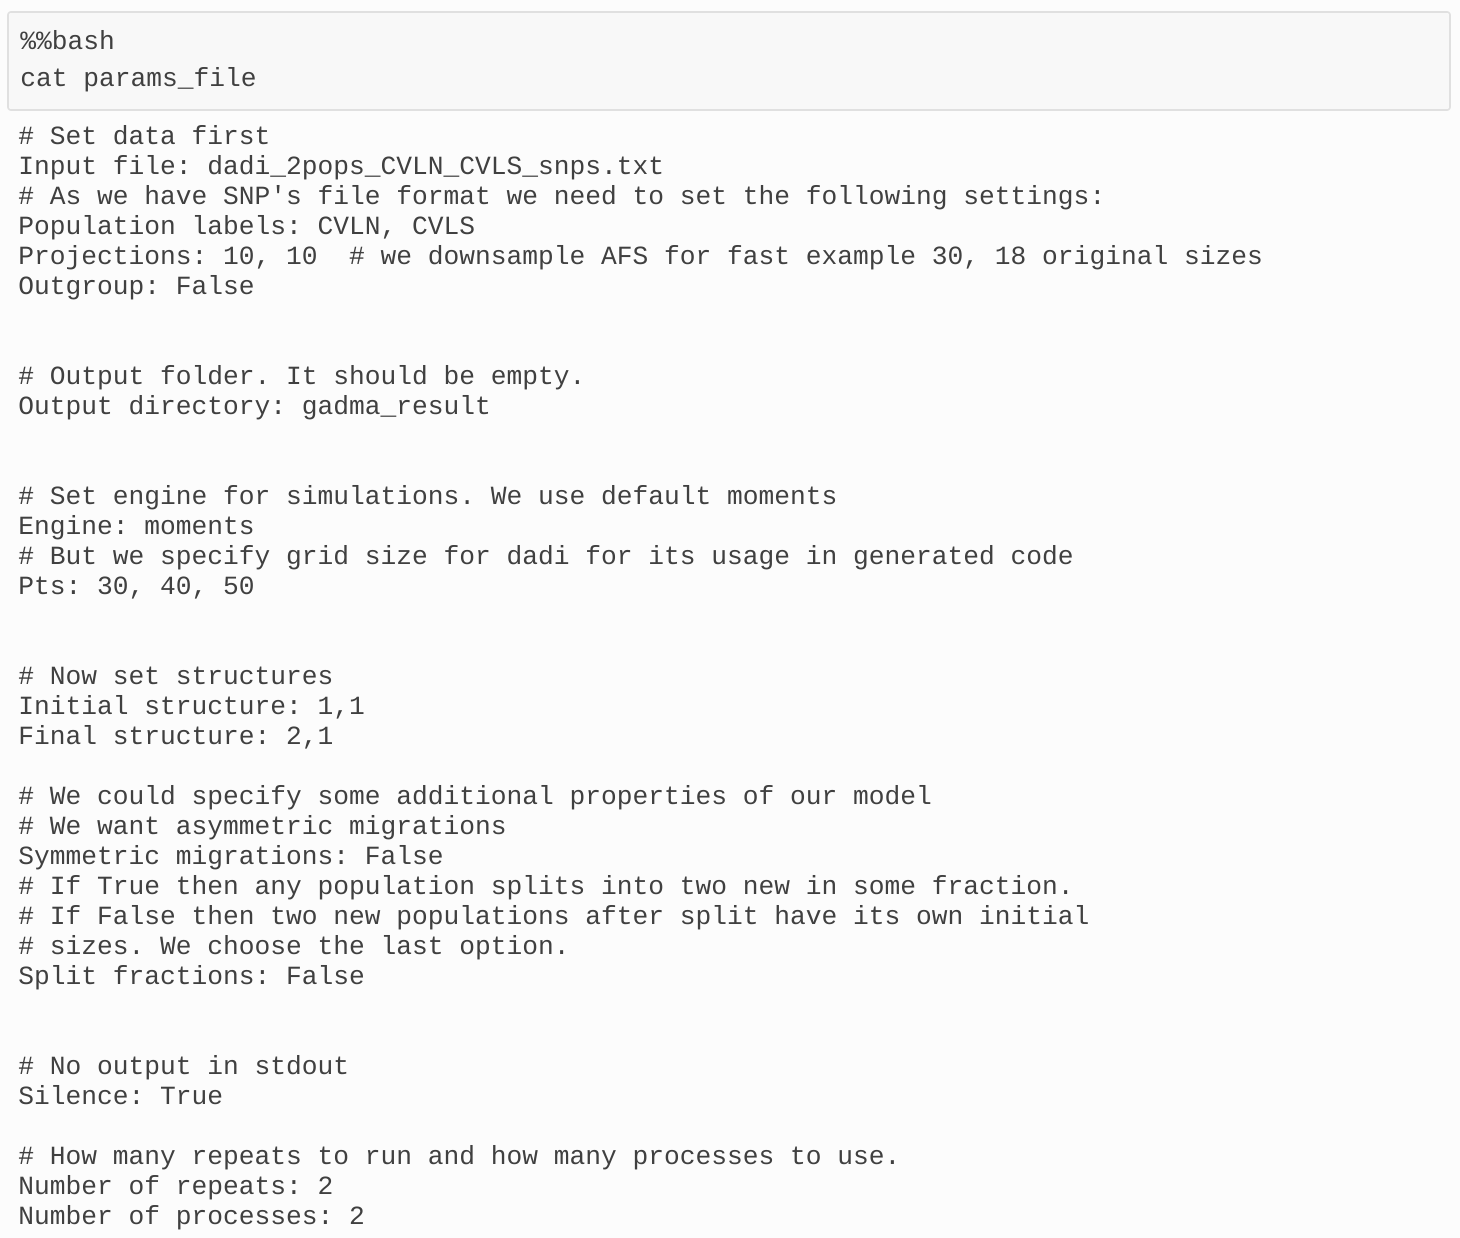
\includegraphics[width=0.9\linewidth]{images/part5/input_file_example.png}
    \caption{Пример входного файла с опциями запуска для программного комплекса GADMA}
    \label{fig:part5:input_example}
\end{figure}

\subsection{Выходные данные}

Все промежуточные и конечные результаты работы программного комплекса GADMA записываются и сохраняются в указанную пользователем директорию (\texttt{Output directory}).
Пример структуры этой директории показан на рисунке~\ref{fig:part5:directory}.
GADMA позволяет вывести демографическую историю популяций, используя несколько запусков-повторов и выбор наилучшего результата.
В основной директории создаются пронумерованные папки, которые содержат результаты каждого повтора.
Например, запуск GADMA, выходные данные которого показаны на рисунке~\ref{fig:part5:directory}, содержал два повтора вывода демографической истории.
В основную часть сохраняется наилучший результат среди повторов.

\begin{figure}[!htbp]
    \centering
    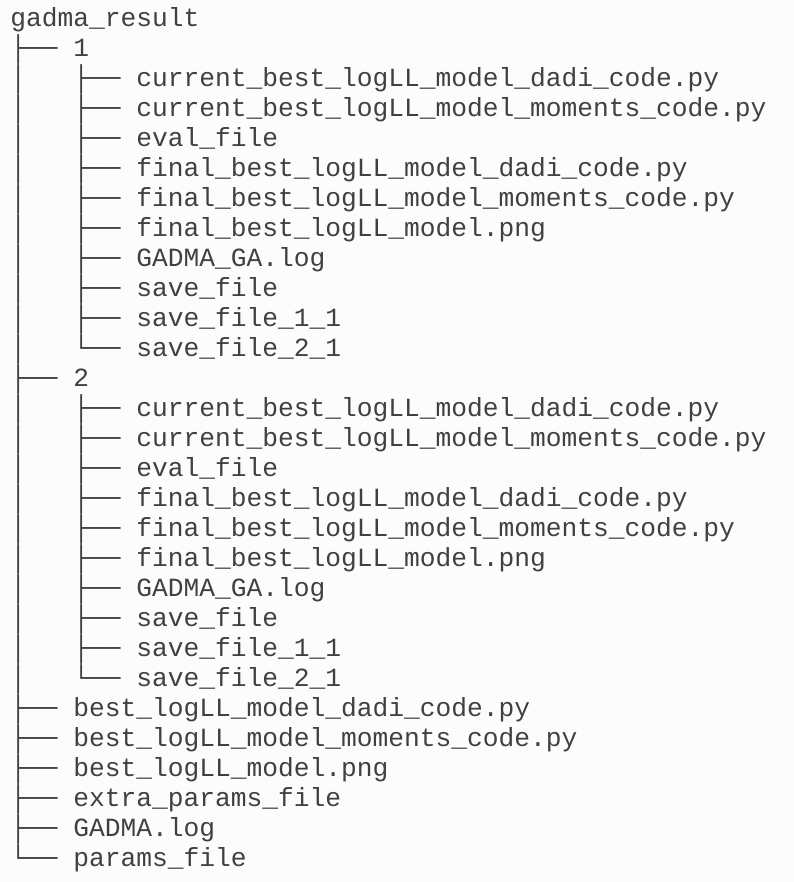
\includegraphics[width=0.5\linewidth]{images/part5/directory_example.png}
    \caption{Пример структуры директории с результатами запуска}
    \label{fig:part5:directory}
\end{figure}

Для полученной демографической истории в директорию записываются текстовое и визуальное представление.
Текстовое представление генерируется для всех доступных движков, например, на рисунке~\ref{fig:part5:directory} файлы \texttt{best\_logLL\_model\_dadi\_code.py} и \texttt{best\_logLL\_model\_dadi\_code.py} являются текстовым представлением полученной демографической истории для \dadi и \moments соответственно.
Визуальное представление демографической истории представлено в файле \texttt{best\_logLL\_model.png}, оно включает изображение демографической истории, сгенерированное одним из движков, а также представление использованных статистик генетических данных.
На рисунке~\ref{fig:part5:png_plot} приведен пример выходного визуального изображения.

\begin{figure}[!htbp]
    \centering
    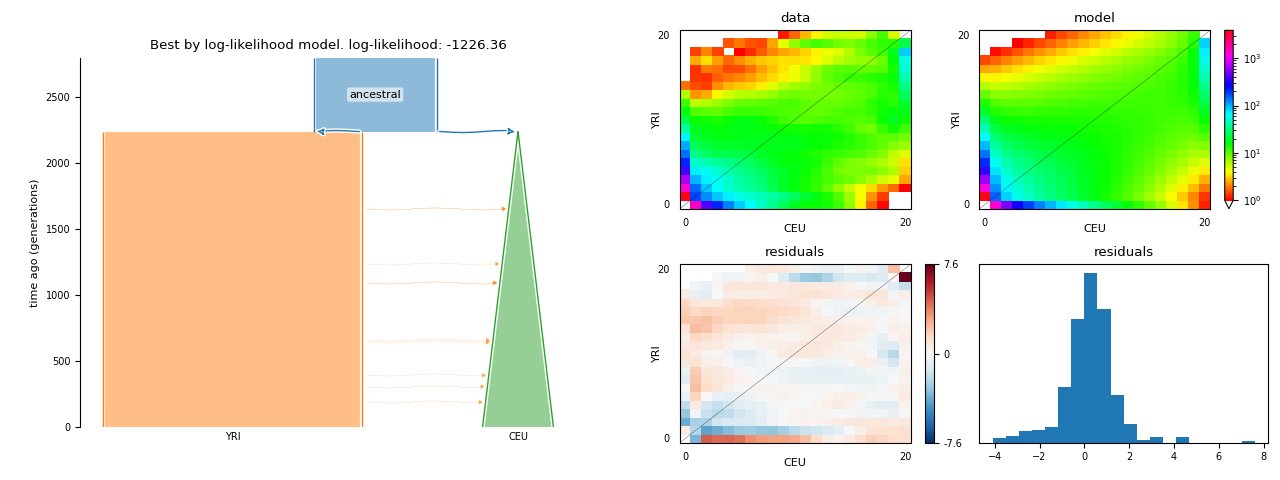
\includegraphics[width=\linewidth]{images/part5/example_model_plot_demes.png}
    \caption{Пример визуального представления демографической истории популяций и использованных статистик генетических данных, созданное GADMA}
    \label{fig:part5:png_plot}
\end{figure}

Запуск GADMA происходит из командной строки, где также выводится информация о результатах запуска.
Пример вывода GADMA в командной строке показан на рисунке~\ref{fig:part5:output_example}.

\begin{figure}[!htbp]
    \centering
    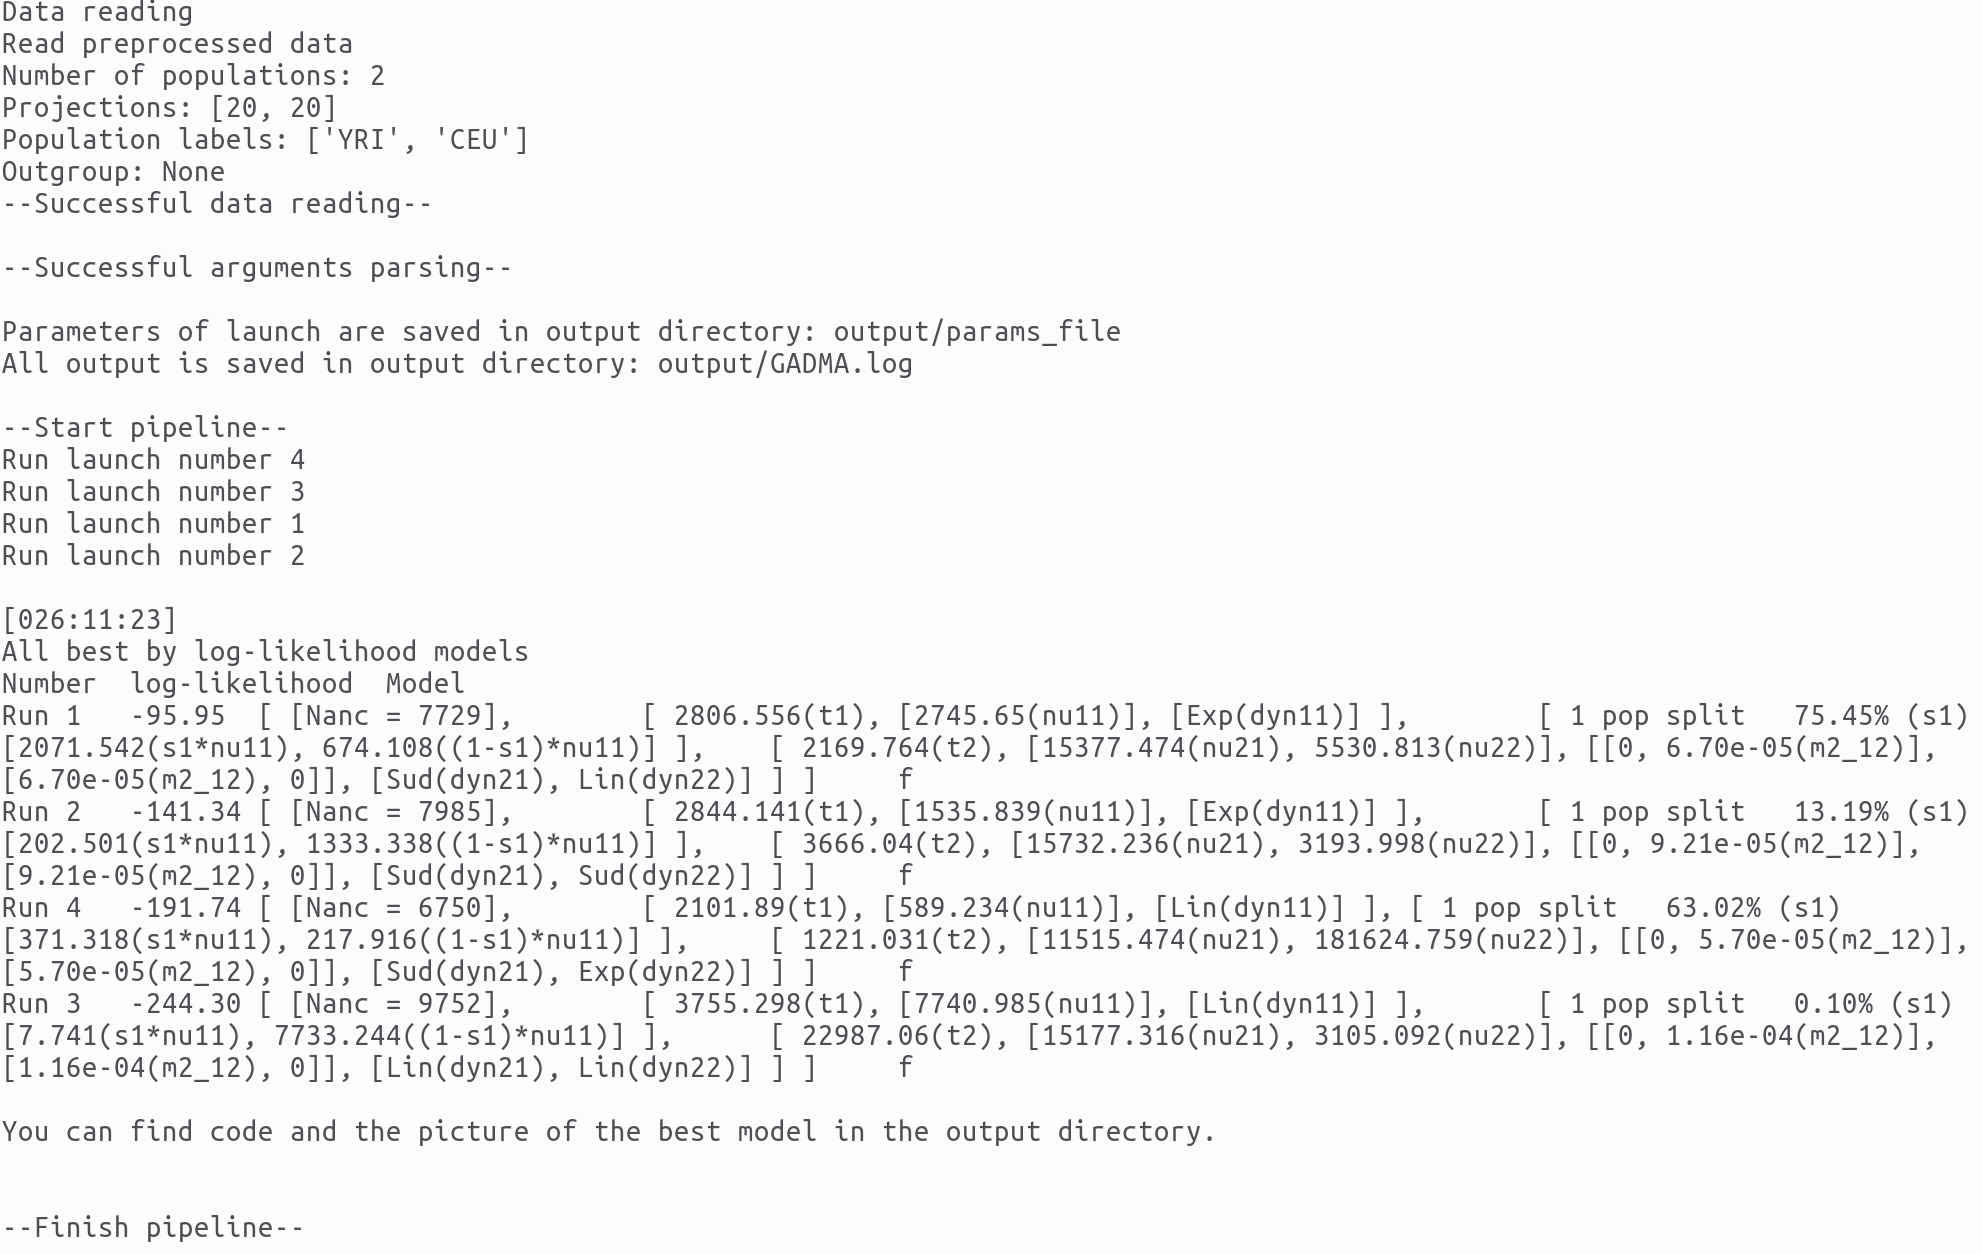
\includegraphics[width=\linewidth]{images/part5/output_example.png}
    \caption{Пример вывода GADMA в командной строке}
    \label{fig:part5:output_example}
\end{figure}

\FloatBarrier
\textbf{Функциональные ограничения на применение.}
При использовании метода автоматического перебора моделей вывод демографической истории в GADMA ограничен тремя популяциями в силу ограничений самого метода.
В случае режима настройки параметров заданной модели демографической истории популяций программный комплекс GADMA ограничен применимостью методов вычисления правдоподобия включенных движков.
Так, например, движки \dadi и \moments могут анализировать до трех и пяти популяций соответственно, а метод вычисления правдоподобия, реализованный в \momi, не поддерживает непрерывные миграции.
Движок \dadi является единственным движком, поддерживающим вывод коэффициентов инбридинга.
Полный список ограничений движков представлен в таблице~\ref{tab:part5:limitations}.

\begin{table}[ht]
    \centering
    \resizebox{\linewidth}{!}{%
    \begin{tabular}{|l|c|c|c|c|}
        \hline
         & \dadi &\moments & \momi & \momentsLD \\
        \hline
        Максимальное число популяций & Три & Пять & Произвольное & Произвольное \\
        в режиме заданной модели & & & & \\
        \hline
        Максимальное число популяций & Три & Три & Три & Три \\
        в режиме автоматического перебора & & & & \\
        \hline
        Учитывает степень рекомбинации & Нет & Нет & Нет & Да \\
        \hline
        Поддерживает линейное & Да & Да & Нет & Да \\
        изменение численности & & & &\\
        \hline
        Поддерживает вывод непрерывной & Да & Да & Нет & Да \\
        миграции & & & &\\
        \hline
        Поддерживает вывод коэффициентов & Да & Нет & Нет & Нет \\
        инбридинга & & & & \\
        \hline
    \end{tabular}%
    }
    \caption{Ограничения программного комплекса GADMA при использовании разных движков}
    \label{tab:part5:limitations}
\end{table}

%\FloatBarrier
\vspace{-0.5cm}
\subsection{Разработка и сопровождение программного комплекса}

Исходный код программного комплекса GADMA находится в \textbf{открытом доступе} на GitHub под лицензией GPLv3: \url{https://github.com/ctlab/GADMA}.
При разработке была использована распределённая система управления версиями (git), что позволило привлечь группу специалистов к совместной работе над проектом.
Всего в разработке программного комплекса приняли участие семь человек.
Разработчиком, внесшим наибольший вклад (более 85 \%), является диссертант, остальные участники --- студенты, которые выполняли работу под руководством диссертанта.
%На рисунке~\ref{fig:part5:charts} показан вклад каждого из участника разработки в обновление рабочей копии проекта (commit) и в программный код последней версии GADMA.

% \begin{figure}[!htbp]
%     \centering
%     \begin{subfigure}[b]{.49\textwidth}
%     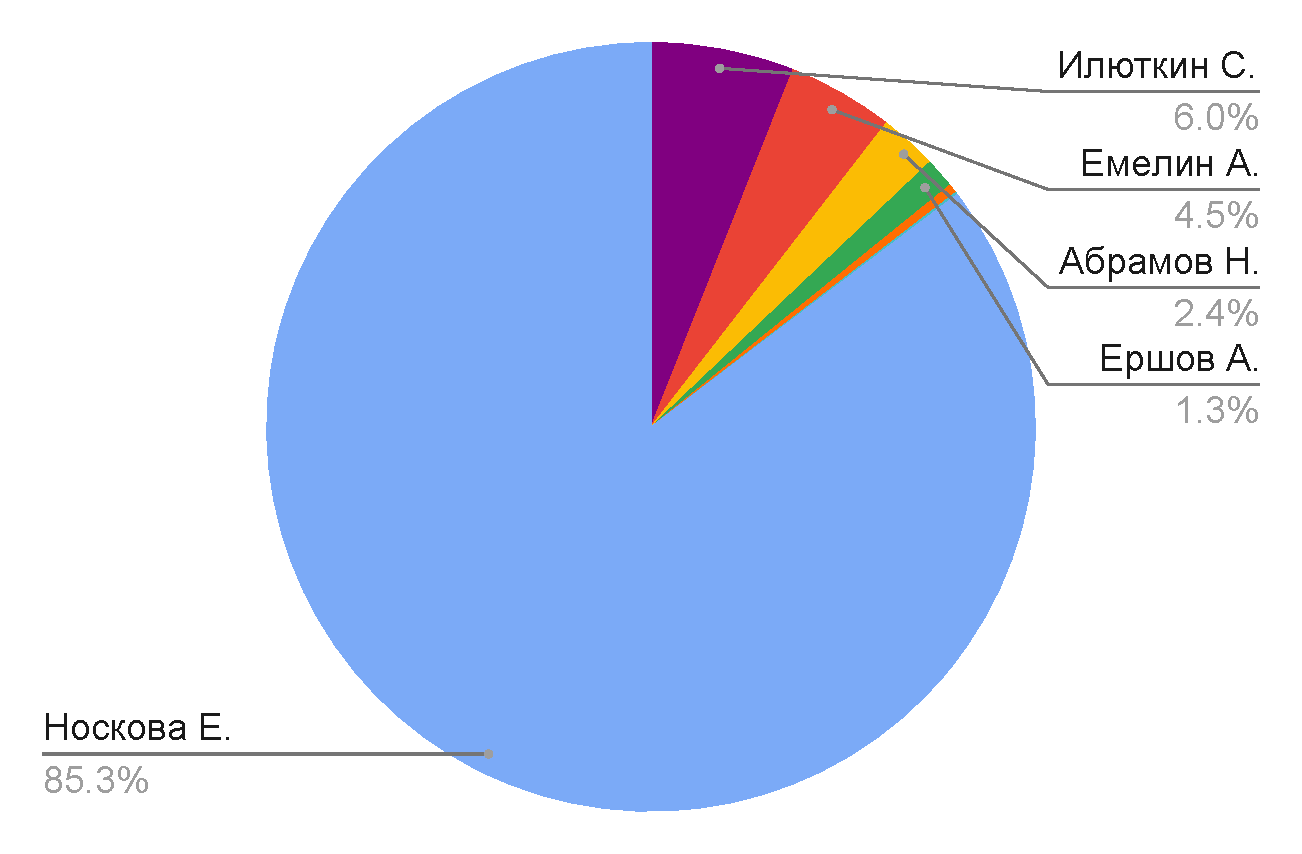
\includegraphics[width=\textwidth]{images/part5/commits.pdf}
%     \caption{}
%     \label{fig:part5:charts:commits}
%     \end{subfigure}%
%     \begin{subfigure}[b]{.49\textwidth}
%     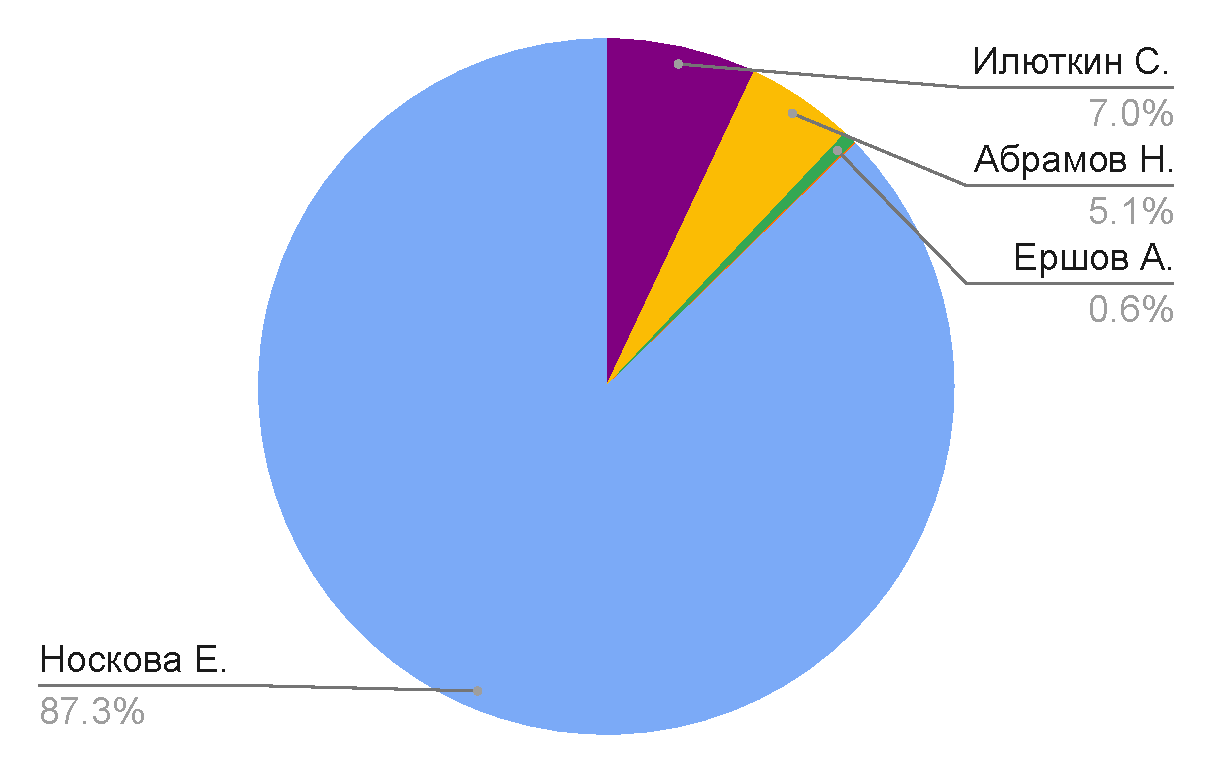
\includegraphics[width=\textwidth]{images/part5/code.pdf}
%     \caption{}
%     \label{fig:part5:charts:code}
%     \end{subfigure}
%     \caption{Вклад участников разработки (а) в обновление рабочей копии проекта, (б) программный код последней версии GADMA}
%     \label{fig:part5:charts}
% \end{figure}

Веб-сервис GitHub позволил осуществлять сопровождение программного комплекса за счет использования \textbf{системы отслеживания ошибок} (issue).
Это позволило обнаружить и исправить ряд дефектов программного комплекса, а также получить отзывы и пожелания внешних участников.

\textbf{Публичные версии программного комплекса} доступны в каталоге \textit{PyPI} (Python Package Index) программного обеспечения, написанного на языке программирования Python, и в дистрибутиве \textit{Anaconda}.
Это означает, что GADMA может быть легко установлена вместе с зависимостями с помощью команд \textit{pip} и \textit{conda} в терминале.

Была использована \textbf{система автоматизации \textit{GitHub Actions}} для программного комплекса GADMA.
\textit{GitHub Actions} --- система непрерывной интеграции и непрерывного развертывания, которая позволяет выполнить сборку, тестирование и публикацию кода программного обеспечения.

\textbf{Общедоступная документация} была создана с использованием генератора документации \textit{Sphinx}, который позволяет на основе  файлов, представленных в формате reStructuredText построить документацию в формате HTML для дальнейшего размещения в сети интернет.
Документация включает в себя подробное описание установки и использования программного комплекса, набор примеров использования и полученных результатов, список частозадаваемых вопросов с ответами и список ссылок на исследовательские работы.
Кроме того, GADMA является библиотекой и может быть использована для решения задач в других областях, где возникает задача оптимизации, поэтому документация включает автоматически созданную документацию интерфейса прикладного программирования (API) GADMA, в которой описаны основные классы.
При каждом обновлении кодовой базы проекта система \textit{GitHub Actions} автоматически создает документацию в формате HTML и размещает новую версию в сети интернет по ссылке:~\url{https://gadma.readthedocs.io}.

Для программного комплекса GADMA была обеспечена возможность проведения \textbf{модульного тестирования} (unit testing).
Тесты могут быть запущены локально с использованием исходного кода, однако их основное назначение --- автоматическое тестирование в системе \textit{GitHub Actions} на различных платформах при обновлении кодовой базы.
Система \textit{GitHub Actions} автоматически собирает комплекс и запускает тесты для следующих платформ: Linux, Windows, MacOS.
По результатам автоматического тестирования создается отчет о покрытии кода тестами.
Этот отчет загружается на сервис \textit{CodeCov}, где он является общедоступным по ссылке:~\url{https://app.codecov.io/gh/ctlab/GADMA}.
Покрытие кода последней версии GADMA составило $96{,}65$\% и пример отчета, доступного на сервисе \textit{CodeCov}, показан на рисунке~\ref{fig:part5:codecov}.

\begin{figure}[ht]
    \centering
    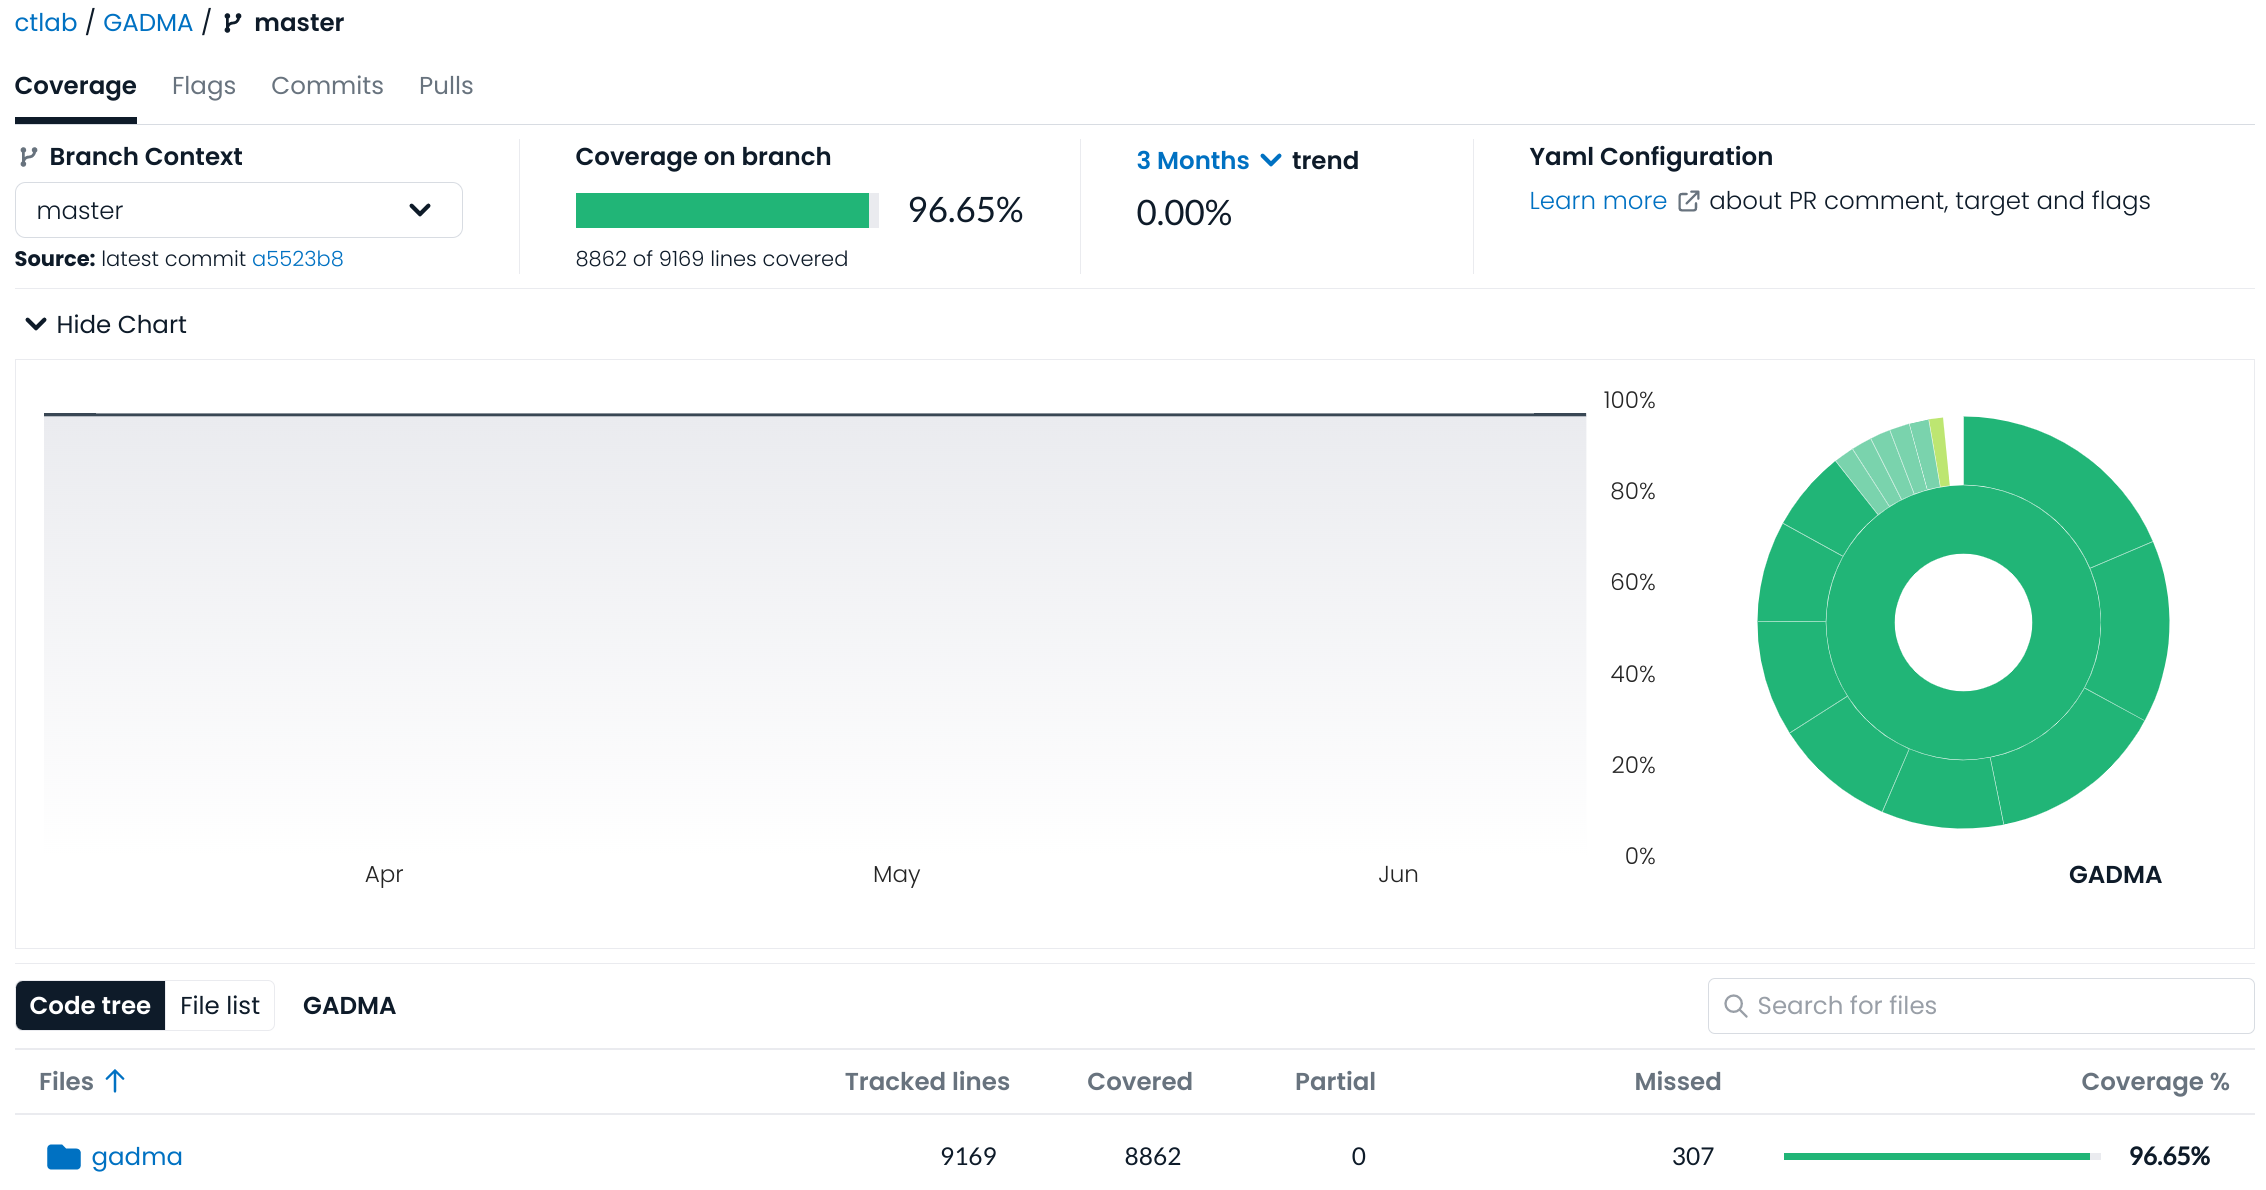
\includegraphics[width=\linewidth]{images/part5/codecov_report.png}
    \caption{Пример отчета о покрытии программного кода GADMA тестами на сервисе \textit{CodeCov}}
    \label{fig:part5:codecov}
\end{figure}

% Вклад участников разработки GADMA в создание документации и тестов показан на рисунке~\ref{fig:part5:charts_2}.

% \begin{figure}[!htbp]
%     \centering
%     \begin{subfigure}[b]{.49\textwidth}
%     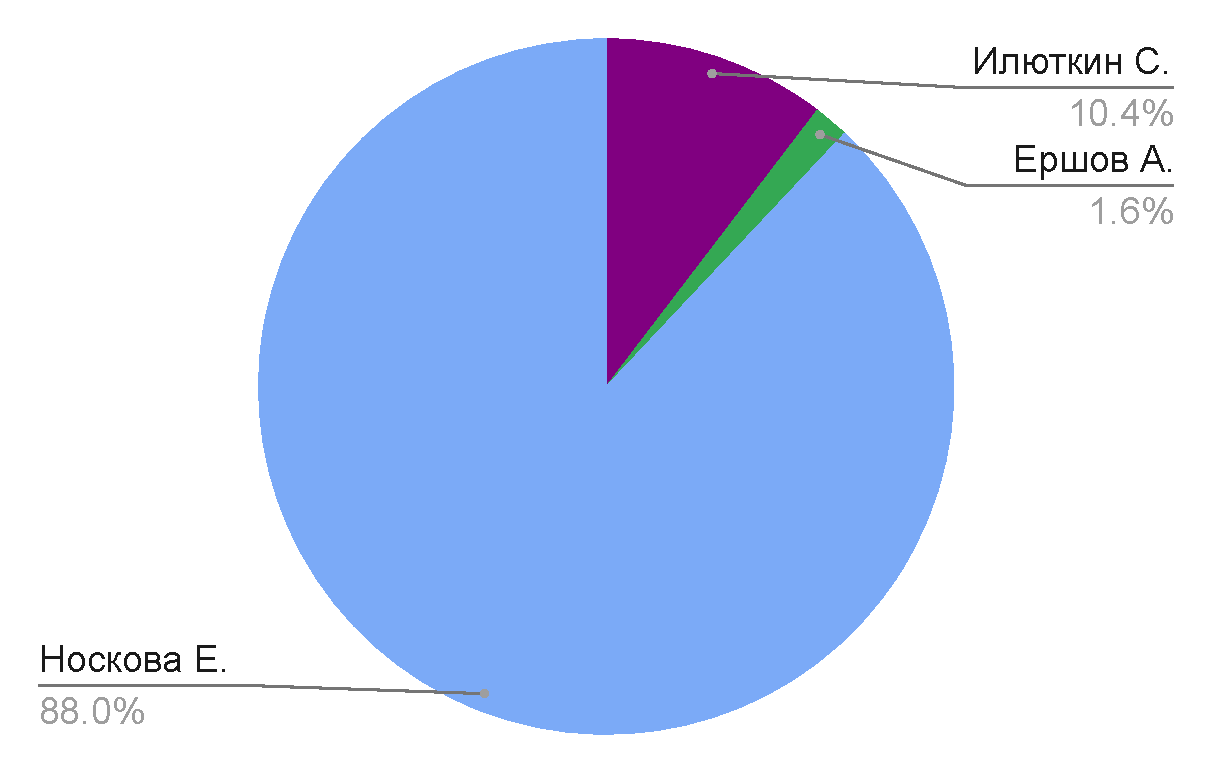
\includegraphics[width=\textwidth]{images/part5/docs.pdf}
%     \caption{}
%     \label{fig:part5:charts:documentation}
%     \end{subfigure}%
%     \begin{subfigure}[b]{.49\textwidth}
%     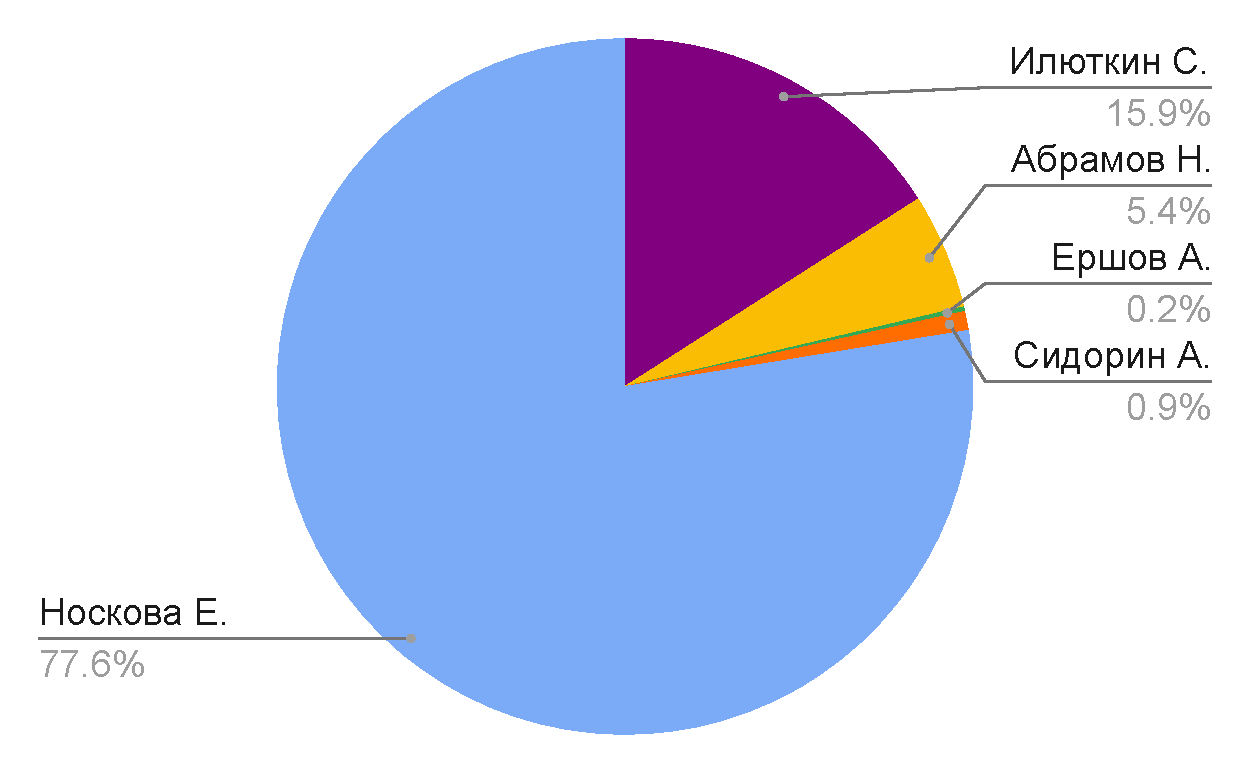
\includegraphics[width=\textwidth]{images/part5/tests.pdf}
%     \caption{}
%     \label{fig:part5:charts:tests}
%     \end{subfigure}
%     \caption{Вклад участников разработки в (а)~создание документации, (б)~создание тестов}
%     \label{fig:part5:charts_2}
% \end{figure}

\FloatBarrier
\section{Расширение библиотек \textit{stdpopsim} и \textit{demes} для проведения экспериментальных исследований и представления результатов}

В данном разделе описаны основные изменения, сделанные для расширения библиотек \textit{stdpopsim} и \textit{demes}.
Эти библиотеки были использованы при проведении экспериментальных исследований в данной работе, библиотека \textit{demes} была также использована для визуального представления демографических историй.

\subsection{Расширение библиотеки \textit{stdpopsim} для симулирования генетических данных}

Библиотека \textit{stdpopsim} --- поддерживаемая сообществом PopSim библиотека стандартных моделей популяционной генетики для симулирования генетических данных~\cite{adrion2020community,lauterbur2023expanding}.
Библиотека предоставляет каталог существующих биологических видов (рисунок~\ref{fig:part5:stdpopsim}).
Для каждого биологического вида представлена информация о геноме --- число хромосом, длина хромосом, и другая информация, которая используется в популяционной генетике --- скорость мутации, вероятности рекомбинации, карты рекомбинации.
Для многих видов представлены демографические истории, ранее полученные в опубликованных исследованиях.

\begin{figure}[ht]
    \centering
    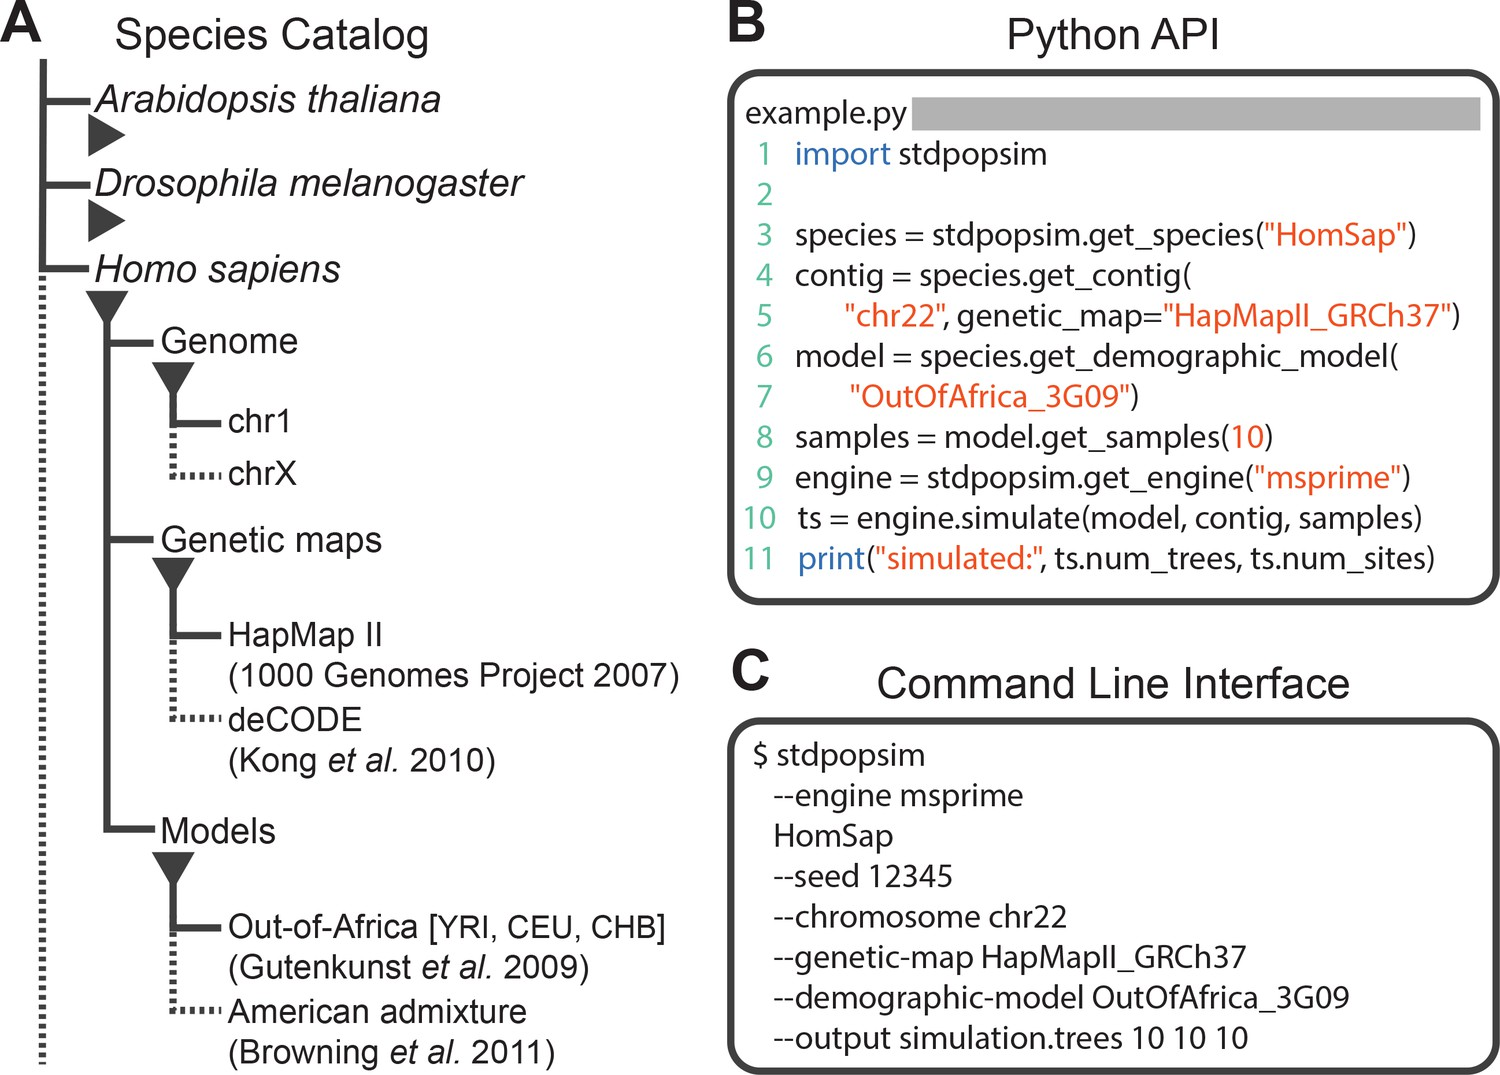
\includegraphics[width=0.9\linewidth]{images/part5/stdpopsim.jpg}
    \caption{Иерархическая структура каталога библиотеки \textit{stdpopsim}, интерфейс прикладного программирования (API) и интерфейс командной строки. Источник:~\cite{adrion2020community}}
    \label{fig:part5:stdpopsim}
\end{figure}

Библиотека позволяет легко проводить симуляции для целого ряда организмов.
\textit{Stdpopsim} имеет интерфейс прикладного программирования (API) на языке Python и удобный интерфейс командной строки, что позволяет пользователям с минимальным опытом программирования использовать эту библиотеку.
Симуляции выполняются с применением одного из двух методов: \textit{msprime}~\cite{kelleher2016efficient}, SLiM~\cite{haller2019slim}.
Пользователю достаточно выбрать метод симуляции, вид организмов, демографическую историю и число образцов и получить симулированные генетические данные.

Библиотека имеет открытый исходный код, доступный по адресу~\url{https://github.com/popsim-consortium/stdpopsim} и общедоступную документацию: \url{https://popsim-consortium.github.io/stdpopsim-docs}.
Разработка ведется широкой группой разработчиков-исследователей с использованием веб-сервиса GitHub с непрерывной интеграцией.
На момент 2023 года число участников проекта насчитывает больше 50.
При расширении каталога библиотеки используется система двойной проверки или контроля качества: сначала один участник проекта добавляет объект --- биологический вид или демографическую историю, затем другой участник выполняет добавление того же объекта независимо (quality control).
Автоматическая система сравнивает оба объекта и, в случае их совпадения, они добавляются в кодовую базу каталога библиотеки.
Такой подход позволяет выполнять контроль качества и избегать ошибок разработки.

Автором диссертации был внесен следующий вклад в разработку и расширение библиотеки \textit{stdpopsim}:
\begin{itemize}
    \item добавление биологического вида \textit{Heliconius melpomene} в каталог (контроль качества): \url{https://github.com/popsim-consortium/stdpopsim/pull/1165};
    \item добавление демографической истории \texttt{PapuansOutOfAfrica\_10J19} десяти популяций современного человека для биологического вида \textit{Homo Sapiens} в каталог (контроль качества): \url{https://github.com/popsim-consortium/stdpopsim/pull/387};
    \item добавление демографической истории \texttt{African3Epoch\_1H18} для биологического вида \textit{Arabidopsis thaliana} в каталог: \url{https://github.com/popsim-consortium/stdpopsim/pull/270};
    \item тестирование библиотеки и выявление дефектов, публикация описания дефектов в системе отслеживания ошибок: \url{https://github.com/popsim-consortium/stdpopsim/issues/701};
    \item добавление документации: \url{https://github.com/popsim-consortium/stdpopsim/pull/333}.
\end{itemize}

Библиотека \stdpopsim была применена для симулирования данных при проведении экспериментальных исследований разработанного метода настройки параметров моделей на основе комбинации генетического алгоритма и локального поиска, которые представлены в разделе~\ref{sec:part2:ga_experiments:orangutan}.

\subsection{Расширение библиотеки \textit{demes} для текстового и визуального представления демографических историй}

Библиотека \textit{demes} позволяет построить и использовать текстовое и визуальное представление демографических историй.
Библиотека также была разработана сообществом PopSim, как и библиотека \textit{stdpopsim}.
В проекте по разработке принимали участие семь участников.
Тестовое представление реализовано в широко используемом формате YAML~\cite{ben2009yaml}, который является языком сериализации данных, обеспечивающим хороший баланс между человеческой и машинной читабельностью.
Спецификация гарантирует отсутствие двусмысленности интерпретации.
Общедоступная документация включает в себя обширный набор тестовых примеров и их ожидаемый результат.
Пример текстового и соответствующего визуального представления для демографической истории представлено на рисунке~\ref{fig:part5:demes_example}.

\begin{figure}[ht]
    \centering
    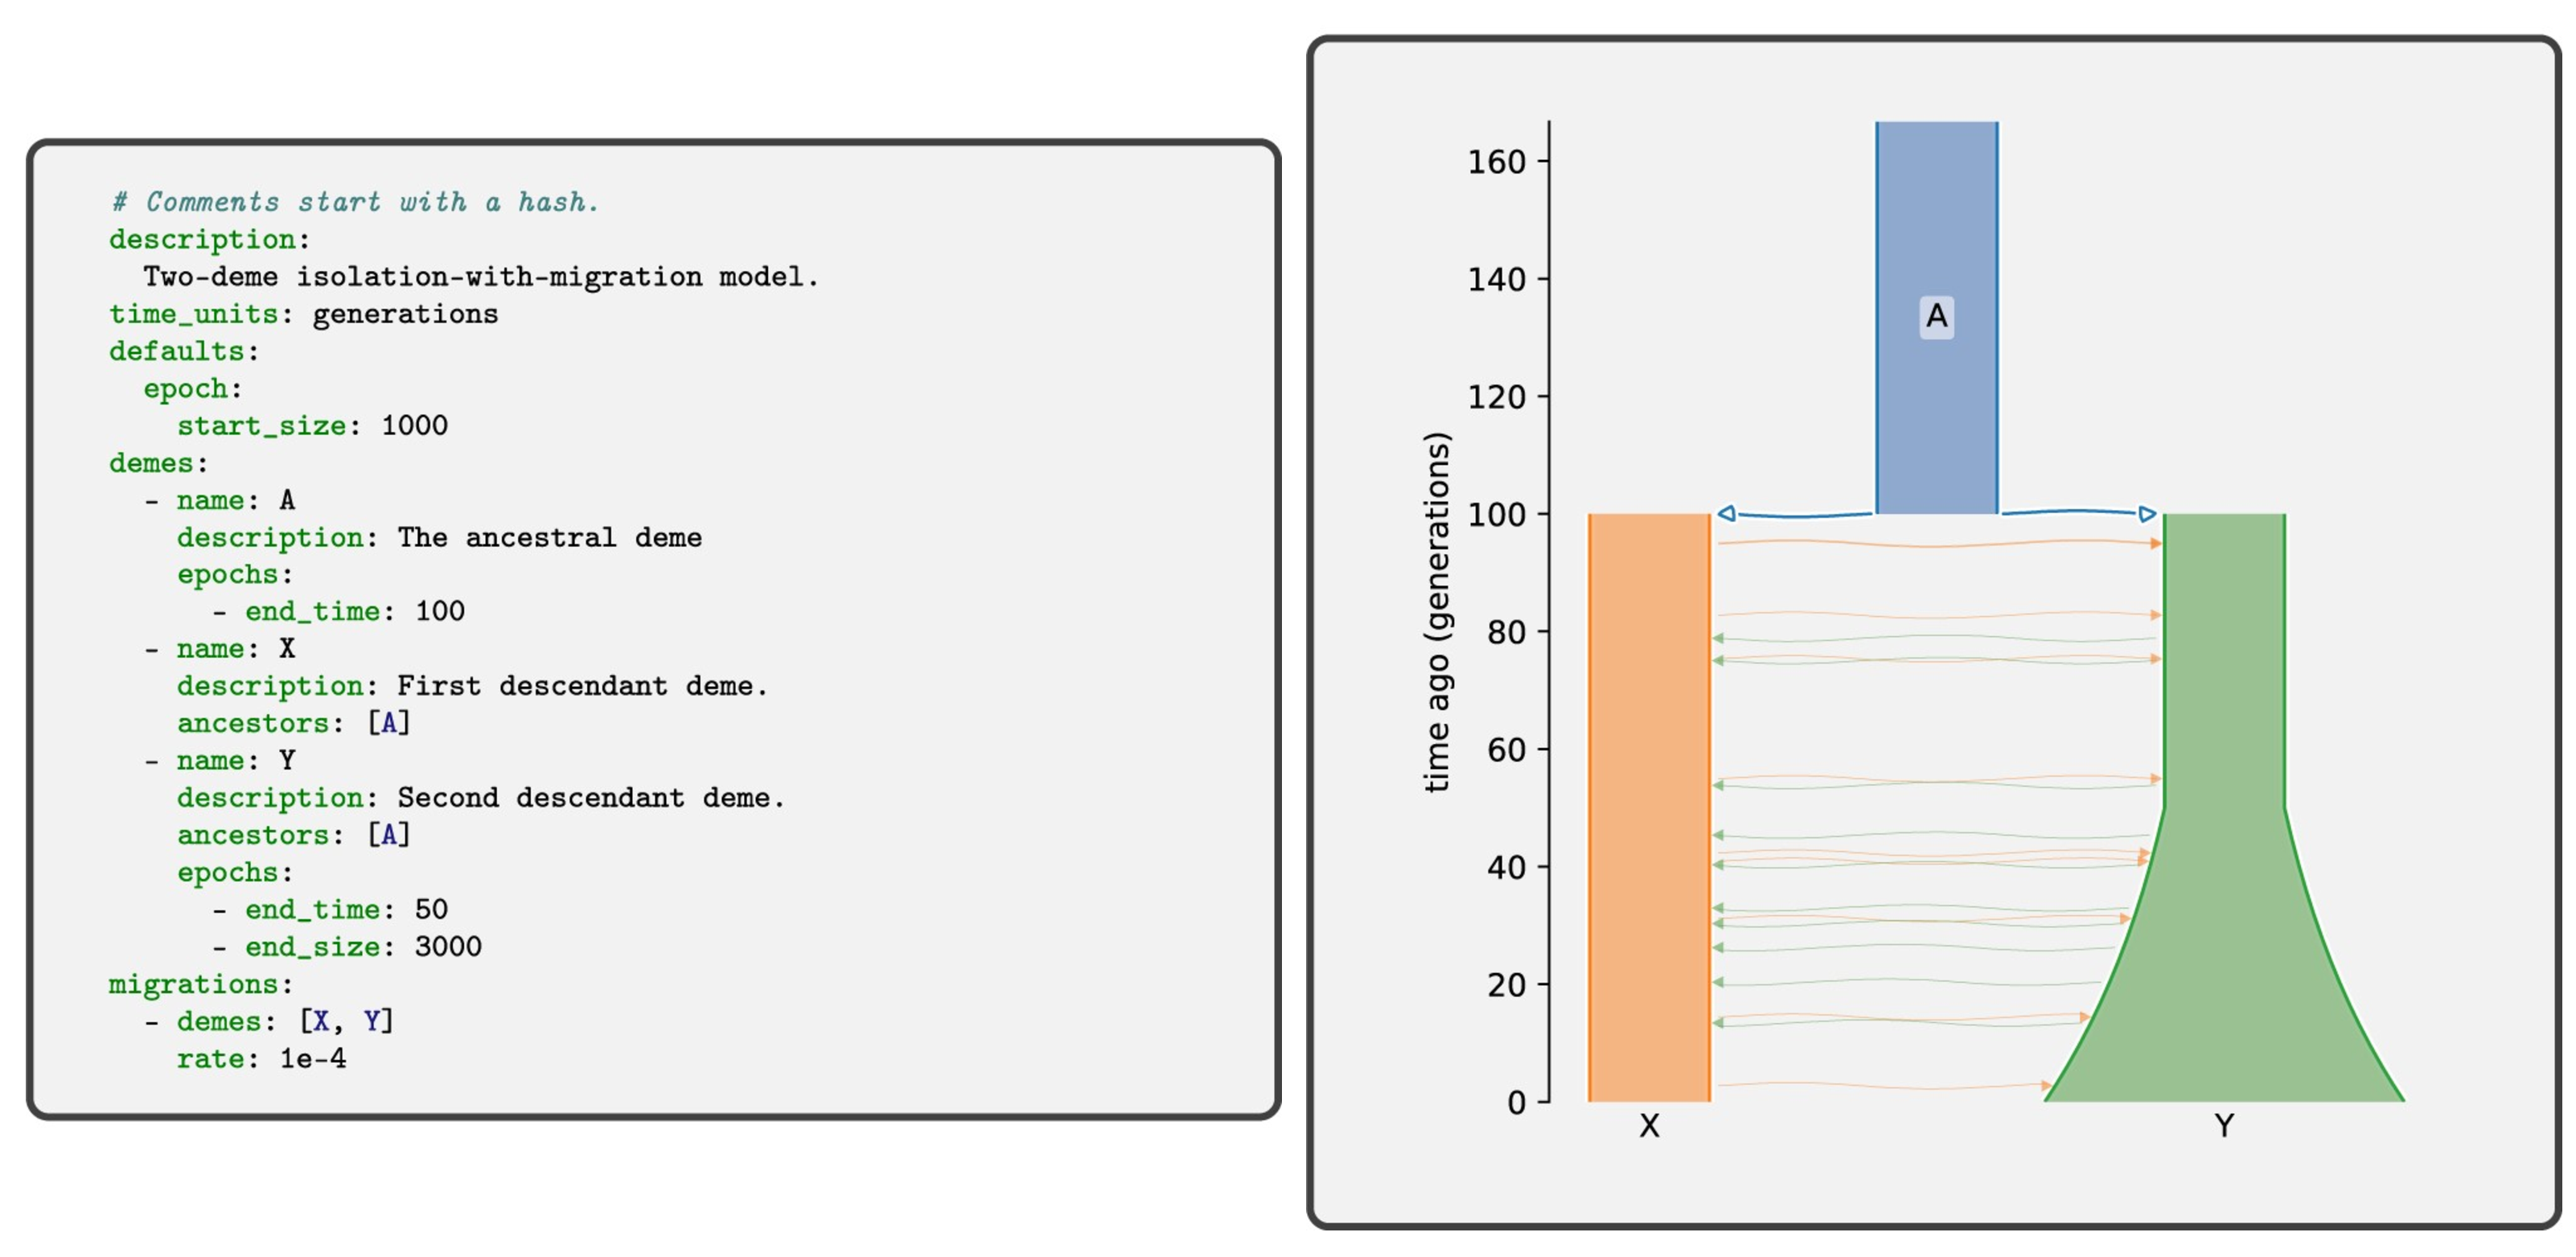
\includegraphics[width=\linewidth]{images/part5/showcase.pdf}
    \caption{Пример тестового и визуального представления демографической истории, полученных с применением \textit{demes}. Источник:~\cite{gower2022demes}}
    \label{fig:part5:demes_example}
\end{figure}

Библиотека имеет открытый исходный код, доступный по адресу~\url{https://github.com/popsim-consortium/demes-python} и общедоступную документацию: \url{https://popsim-consortium.github.io/demes-docs}.

Автором диссертации был внесен следующий вклад в разработку и расширение библиотеки \textit{demes}:
\begin{itemize}
    \item добавление линейной функции изменения численности популяций;
    \item разработка части программного кода библиотеки (5 \%);
    \item интеграция библиотеки \textit{demes} в программный комплекс GADMA.
\end{itemize}


\section*{Выводы по граве~\ref{ch:implementation}}
\addcontentsline{toc}{section}{Выводы по главе~\ref{ch:implementation}}

\begin{enumerate}[label={\arabic*.}]
    \item Описан разработанный программный комплекс GADMA для вывода демографической истории популяций, реализующий разработанные модели и методы. 
    \item Программный комплекс имеет репозиторий с открытым исходным кодом, доступным по адресу~\url{https://github.com/ctlab/GADMA}, общедоступную документацию и систему автоматического тестирования программного кода.
    \item Каталог доступных биологических видов для симуляции данных в библиотеке \textit{stdpopsim} был расширен. Библиотека была протестирована и использована при проведении экспериментальных исследований в данной работе.
    \item Библиотека \textit{demes} позволяет построить текстовое и визуальное представление демографических историй. Библиотека была расширена добавлением линейной динамики изменения численности популяций и была интегрирована в программный комплекс GADMA.
    \item Все визуальные представления демографических историй, представленные в данной работе, получены с применением библиотеки \textit{demes}.
\end{enumerate}